%% (Master) Thesis template
% Template version used: v1.4
%
% Largely adapted from Adrian Nievergelt's template for the ADPS
% (lecture notes) project.


%% We use the memoir class because it offers a many easy to use features.
\documentclass[11pt,a4paper,titlepage,oneside]{memoir}

%% Packages
%% ========

%% LaTeX Font encoding -- DO NOT CHANGE
\usepackage[OT1]{fontenc}

%% Babel provides support for languages.  'english' uses British
%% English hyphenation and text snippets like "Figure" and
%% "Theorem". Use the option 'ngerman' if your document is in German.
%% Use 'american' for American English.  Note that if you change this,
%% the next LaTeX run may show spurious errors.  Simply run it again.
%% If they persist, remove the .aux file and try again.
\usepackage[english]{babel}

%% Input encoding 'utf8'. In some cases you might need 'utf8x' for
%% extra symbols. Not all editors, especially on Windows, are UTF-8
%% capable, so you may want to use 'latin1' instead.
\usepackage[utf8]{inputenc}

%% This changes default fonts for both text and math mode to use Herman Zapfs
%% excellent Palatino font.  Do not change this.
\usepackage[sc]{mathpazo}

%% The AMS-LaTeX extensions for mathematical typesetting.  Do not
%% remove.
\usepackage{amsmath,amssymb,amsfonts,mathrsfs}

%% NTheorem is a reimplementation of the AMS Theorem package. This
%% will allow us to typeset theorems like examples, proofs and
%% similar.  Do not remove.
%% NOTE: Must be loaded AFTER amsmath, or the \qed placement will
%% break
\usepackage[amsmath,thmmarks]{ntheorem}

%% LaTeX' own graphics handling
\usepackage{graphicx}

%% We unfortunately need this for the Rules chapter.  Remove it
%% afterwards; or at least NEVER use its underlining features.
\usepackage{soul}

%% This allows you to add .pdf files. It is used to add the
%% declaration of originality.
\usepackage{pdfpages}

%% Some more packages that you may want to use.  Have a look at the
%% file, and consult the package docs for each.
%\input{extrapackages}

%% Our layout configuration.  DO NOT CHANGE.
%% Memoir layout setup

%% NOTE: You are strongly advised not to change any of them unless you
%% know what you are doing.  These settings strongly interact in the
%% final look of the document.

% Dependencies
\usepackage{ETHlogo}

% Turn extra space before chapter headings off.
\setlength{\beforechapskip}{0pt}

\nonzeroparskip
\parindent=0pt
\defaultlists

% Chapter style redefinition
\makeatletter

\if@twoside
  \pagestyle{Ruled}
  \copypagestyle{chapter}{Ruled}
\else
  \pagestyle{ruled}
  \copypagestyle{chapter}{ruled}
\fi
\makeoddhead{chapter}{}{}{}
\makeevenhead{chapter}{}{}{}
\makeheadrule{chapter}{\textwidth}{0pt}
\copypagestyle{abstract}{empty}

\makechapterstyle{bianchimod}{%
  \chapterstyle{default}
  \renewcommand*{\chapnamefont}{\normalfont\Large\sffamily}
  \renewcommand*{\chapnumfont}{\normalfont\Large\sffamily}
  \renewcommand*{\printchaptername}{%
    \chapnamefont\centering\@chapapp}
  \renewcommand*{\printchapternum}{\chapnumfont {\thechapter}}
  \renewcommand*{\chaptitlefont}{\normalfont\huge\sffamily}
  \renewcommand*{\printchaptertitle}[1]{%
    \hrule\vskip\onelineskip \centering \chaptitlefont\textbf{\vphantom{gyM}##1}\par}
  \renewcommand*{\afterchaptertitle}{\vskip\onelineskip \hrule\vskip
    \afterchapskip}
  \renewcommand*{\printchapternonum}{%
    \vphantom{\chapnumfont {9}}\afterchapternum}}

% Use the newly defined style
\chapterstyle{bianchimod}

\setsecheadstyle{\Large\bfseries\sffamily}
\setsubsecheadstyle{\large\bfseries\sffamily}
\setsubsubsecheadstyle{\bfseries\sffamily}
\setparaheadstyle{\normalsize\bfseries\sffamily}
\setsubparaheadstyle{\normalsize\itshape\sffamily}
\setsubparaindent{0pt}

% Set captions to a more separated style for clearness
\captionnamefont{\sffamily\bfseries\footnotesize}
\captiontitlefont{\sffamily\footnotesize}
\setlength{\intextsep}{16pt}
\setlength{\belowcaptionskip}{1pt}

% Set section and TOC numbering depth to subsection
\setsecnumdepth{subsection}
\settocdepth{subsection}

%% Titlepage adjustments
\pretitle{\vspace{0pt plus 0.7fill}\begin{center}\HUGE\sffamily\bfseries}
\posttitle{\end{center}\par}
\preauthor{\par\begin{center}\let\and\\\Large\sffamily}
\postauthor{\end{center}}
\predate{\par\begin{center}\Large\sffamily}
\postdate{\end{center}}

\def\@advisors{}
\newcommand{\advisors}[1]{\def\@advisors{#1}}
\def\@department{}
\newcommand{\department}[1]{\def\@department{#1}}
\def\@thesistype{}
\newcommand{\thesistype}[1]{\def\@thesistype{#1}}

\renewcommand{\maketitlehooka}{\noindent\ETHlogo[2in]}

\renewcommand{\maketitlehookb}{\vspace{1in}%
  \par\begin{center}\Large\sffamily\@thesistype\end{center}}

\renewcommand{\maketitlehookd}{%
  \vfill\par
  \begin{flushright}
    \sffamily
    \@advisors\par
    \@department, ETH Z\"urich
  \end{flushright}
}

\checkandfixthelayout

\setlength{\droptitle}{-48pt}

\makeatother

% This defines how theorems should look. Best leave as is.
\theoremstyle{plain}
\setlength\theorempostskipamount{0pt}

%%% Local Variables:
%%% mode: latex
%%% TeX-master: "thesis"
%%% End:


%% Helpful macros.
%\input{macrosetup}

%% Make document internal hyperlinks wherever possible. (TOC, references)
%% This MUST be loaded after varioref, which is loaded in 'extrapackages'
%% above.  We just load it last to be safe.
\usepackage[linkcolor=black,colorlinks=true,citecolor=black,filecolor=black]{hyperref}


%% Document information
%% ====================

\title{ArmWrestling: efficient binary rewriting for ARM}
\author{Luca Di Bartolomeo}
\thesistype{Master Thesis}
\advisors{Advisor: Prof.\ Dr.\ Mathias Payer\\Supervisor: Prof.\ Dr.\ Kenny Paterson}
\department{Applied Cryptography Group\\Institute of Information Security\\Department of Computer Science}
\department{Applied Cryptography Group\\Institute of Information Security\\Department of Computer Science}
\date{\today}


\usepackage{xcolor} 
\usepackage{soul}
\usepackage{hyperref}
\usepackage{listings} 
\usepackage{caption}
\usepackage{booktabs}
\usepackage{siunitx}
\usepackage{bm}
\usepackage{xspace}


\usepackage[
  backend=biber,
  style=numeric-comp,
  hyperref=true,
  %style=numeric,
  %sorting=ydnt,
  defernumbers=true,
  maxbibnames=99,
]{biblatex}
\addbibresource{thesis.bib}

\definecolor{lgray}{rgb}{0.92,0.92,0.92}
\definecolor{dgray}{rgb}{0.46,0.46,0.46}

\lstset{ %
  language=[x86masm]Assembler,    
  framexleftmargin=5pt,
  framexrightmargin=5pt,
  %framesep=100pt,
  basicstyle=\ttfamily\small,      
  numbers=none,                  
  numberstyle=\small\color{gray},  
  numbersep=15pt,
  stepnumber=1,                   
  backgroundcolor=\color{lgray},  
  tabsize=4,                      
  captionpos=b,                   
  breaklines=true,               
  breakatwhitespace=false,      
  title=\lstname,              
  keywordstyle=\color{blue},     
  commentstyle=\color{dgray}, 
  stringstyle=\color{mauve},   
  escapeinside={\%*}{*)},     
  columns=fullflexible,
  morekeywords={adrp, add, adr, ldrb, br, uxtw, sxtb, b.eq, b.hi, ldr, movz}
}

%\title{Arm Wrestling: efficient binary rewriting on ARM}
%\author{Luca Di Bartolomeo} \adviser{Prof. Mathias Payer (EPFL)}
%\supervisor{Prof. Kenny Paterson (ETH)}

\linespread{1.5} 
\newcommand{\sysname}{RetroWrite-ARM\xspace}
\newcommand{\sysnameold}{RetroWrite-x64\xspace}


\DeclareRobustCommand{\todo}[1]{{\sethlcolor{cyan}\hl{TODO: #1}}}
\DeclareRobustCommand{\mat}[1]{{\sethlcolor{red}\hl{MAT: #1}}}

\begin{document}


\frontmatter

%% Title page is autogenerated from document information above.  DO
%% NOT CHANGE.
\begin{titlingpage}
  \calccentering{\unitlength}
  \begin{adjustwidth*}{\unitlength-24pt}{-\unitlength-24pt}
	\maketitle
  \end{adjustwidth*}
\end{titlingpage}



\clearpage
\renewcommand{\abstractname}{}
\begin{abstract}


\vspace*{4cm}
This thesis was developed with the guidance of prof.Mathias Payer and the
	HexHive research group at EPFL, and under the remote supervision of prof.
	Kenneth Paterson at ETH.
\end{abstract}



\clearpage
\renewcommand{\abstractname}{}
\begin{abstract}

\thispagestyle{empty}
\begin{flushright}
	No matter where you go, everyone is connected.\\
	--- Serial Experiments Lain\\
\end{flushright} 

\vspace*{4cm}
Dedicated to my parents, my brothers Sara and Leo, my dear Giulia, to my friends back 
in Rome and to my roommates Matteo and Filippo who all inspired me and kept 
up with my constant complaining. Thanks!
\end{abstract}



\clearpage
\renewcommand{\abstractname}{Acknowledgments}
\begin{abstract}
	I would like to thank my advisor, Prof. Mathias Payer, for his support,
	guidance, and for trusting me by assigning me this inspiring project.  I
	admire him a lot and I wish all the best for him, and in particular I hope
	that I can work on many other projects with him.
	
	I would also like to thank his research group, HexHive, as I always found
	myself very welcome there, even if I could visit them only once a week.  
	Those have been six very happy months in which I learned quite a lot of 
	things, and I have to thank prof. Prof. Payer and his doctorate students 
	and researches for it. I wish them all to have a very succesfull career, 
	and I hope we can continue to work together in the future!
	
	Special thanks goes to my family and my friends in Rome. Their support was
	always available, and it has always been a huge pleasure to visit them once
	in a while in Italy. I also need to thank my S.O. Giulia, I felt she was
	always behind my back, keeping a good check on my mental sanity during the
	worst times of the outbreak. My roommates too, Matteo and Filippo, deserve
	a mention here, as their patience and their rubber duck debugging skills
	proved to be fundamental during some nasty debugging sessions.

	Finally, I would also like to mention my CTF team, Flagbot, that made me 
	spend so many weekends without going out but ultimately lead me to meet so 
	many new interesting people, and the teams I had played with occasionally, 
	namely polyglots and TRX. Thanks!
\end{abstract}

\clearpage
\renewcommand{\abstractname}{Abstract}
\begin{abstract}
	Closed source programs are particularly hard to audit for vulnerabilities.
	Moreover, it is often the case that modern security measures and
	mitigations are available only as compiler passes that require possession
	of the source code. Even if there were good recent attempts
	\footnote{\url{https://www.pine64.org/pinephone/}}
	\footnote{\url{https://system76.com/}}
	\footnote{\url{https://puri.sm/products/}}
	at completely avoiding usage or closed source libraries of modules that run
	at privileges higher than we might want (e.g., manufacturer specific kernel
	modules \cite{androidclosed})
	in practice it is almost impossible to restrict our computing to
	exclusively open source and audited software.  It is then of paramount
	importance that we find new ways of securing software without source code.

	Many existing tools were developed to improve the auditability of closed
	source programs, especially aimed at helping the fuzzing process, with
	approaches such as implementing AddressSanitizer (a compiler pass only
	available with the source code) through dynamic instrumentation. However,  
	even state-of-the-art dynamic instrumentation engines incur in prohibitive 
	runtime overhead (10x and more). Static rewriters are increasing in popularity, 
	but they are mostly targeted towards the \texttt{x86} architecture.

	We would like to show that symbolization for ARM binaries 
	is a viable alternative to existing approaches, that has less flexibility 
	(only works on C, position independent binaries) but has
	negligible overhead compared to compiled source code. We present 
	\sysname, a \emph{zero-overhead} static binary rewriter for \texttt{aarch64}
	executables that solves key challenges such as pointer construction
	detection and jump table instrumentation, based on 
	the \sysnameold project.

	Our proof of work implementation of a memory sanitizer instrumentation
	pass has the same functionality of the source-based counterpart, and our
	benchmarks show that it is \todo{xx\%} faster than Valgrind's \texttt{memcheck}.
\mat{Make XX a macro and use it throughout when you refer to that number.}

\end{abstract}


\clearpage

%% TOC with the proper setup, do not change.
\cleartorecto
\tableofcontents
\mainmatter

%% Your real content!
%\input{introduction}
%\input{rules}
%\input{typography}
%\input{sections}







%%%%%%%%%%%%%%%%%%%%%%
\chapter{Introduction}
%%%%%%%%%%%%%%%%%%%%%%
%The introduction is a longer writeup that gently eases the reader into your
%thesis~\cite{dinesh20oakland}. Use the first paragraph to discuss the setting.
%In the second paragraph you can introduce the main challenge that you see.
%The third paragraph lists why related work is insufficient.
%The fourth and fifth paragraphs discuss your approach and why it is needed.
%The sixth paragraph will introduce your thesis statement. Think how you can
%distill the essence of your thesis into a single sentence.
%The seventh paragraph will highlight some of your results
%The eights paragraph discusses your core contribution.
%This section is usually 3-5 pages.

Mobile environments are ubiquitous but often lack security updates, for
example, on Android over 60\% of devices are outdated by at least two
years~\cite{android}. Security testing in mobile environments is extremely
challenging as vendors often release components as binary-only, i.e., without
accompanying source code.  Binaries cannot be readily evaluated by security
analysts, resulting in potentially undiscovered vulnerabilities in this
binary-only modules, which often run with high privileges and are exposed to
the network. Binary rewriting is a process that allows insertion of arbitrary code
(instrumentation) in an already compiled binary without the need to recover its
source code, allowing the insertion of hardening measures that are able to 
substantially reduce the exploitability in the case of a vulnerability.
Binary rewriting is also vital to analysts looking for new vulnerabilities,
as it's an important step in the fuzzing of closed source software. 

Binary rewriters can be split into two main categories: \emph{dynamic} rewriters
, that inject code into the target executable at run-time, and \emph{static} ones
, that transform the executable into a new one with the instrumentation already inserted.
The first kind allow more flexibility, and support a broader range of binaries, but
they insert noticeable overhead during its execution; the static ones instead have a much
smaller footprint in execution time but are only applicable on binaries on which the analysis
without runtime information (static analysis) is successful.

%Binary rewriting allows analysts to work with binary-only modules
%but existing solutions are faced with severe disadvantages of either high
%overhead for dynamic rewriting and limited rewriting capabilities for static
%solutions.

While there is no shortage of \emph{static} rewriters targeted towards the
\texttt{x86} architecture, only a few support \texttt{ARM}. In fact, \texttt{ARM} binaries
require a very different kind of static analysis than \texttt{x86}, and present
many challenges that are not found on \texttt{x86}. Those challenges derive from the
fact that the \texttt{ARM} ISA is fixed-size, and all instructions occupy exactly
4 bytes. Since addresses in the 64 bit space are 8-byte long, they do not fit 
into a single instruction, and executables must ``craft'' addresses in various
ways (storing them in memory at compile time, or using arithmetic expressions to 
construct them). A number of static analysis techniques commonly used on \texttt{x86}
are not usable anymore on \texttt{ARM} for this very reason.
There are a number of \emph{dynamic} rewriters that support \texttt{ARM}, and
they work by running together with the binary to instrument and modifying
it in real time: this allows them to use powerful dynamic analysis techniques to 
recover more information about the binary, but as a side effect they introduce
very large overhead even with very light instrumentation.

Introducing only a small overhead onto an instrumented binary is a very desirable feature to 
have into a binary rewriter, as nowadays the largest use case of binary instrumentation
is the injection of fuzzing hooks and memory sanitization checks in a closed 
source binary to drastically improve the efficiency of modern fuzzing
engines. Using a static binary rewriter versus a dynamic one can when
fuzzing can lead to an order of magnitude more executions per second. 

Fuzzing on the \texttt{ARM} architecture has had very little growth when
compared to \texttt{x86}, and one of the main causes is that the required
instrumentation passes to fuzz are supported only by heavy dynamic binary
rewriters, which lead to low fuzzing performances.
The fact that \texttt{ARM} became popular only very recently, combined with the 
difficulty of performing static analysis on it, are the reasons behind the lack
of advanced static binary rewriters for \texttt{ARM}. In fact, most of the existing
ones rely on simpler techniques (like \emph{trampolines}) that need only 
superficial analysis, but are not flexible and incur in very large overhead. 

Static analysis is the core foundation on many state-of-the-art static binary
rewriters: one of the most recent and successful ones for \texttt{x86\_64} is
RetroWrite~\cite{dinesh20oakland}. It uses a novel technique called
\emph{symbolization}, which is the process of transforming an executable back
to an assembly listing that is \emph{re-assemblable}, where absolute addresses
are substituted with assembly labels (or \emph{symbols}).  Since all addresses
are subsituted with labels, adding custom code (instrumentation) or arbitrary
transformation on existing code is very easy, as the resulting assembly can be
parsed by a generic off-the-shelf assembler into a new, instrumented
executable. 

In this thesis we would like to introduce \sysname, a new, advanced static rewriter 
for \texttt{ARM64} binaries that builds on the original RetroWrite (from now on
referred as \sysnameold) and uses the same \emph{symbolization} technique 
to allow the development of complex and efficient instrumentation and trasformation
of closed-source binaries. Our work focuses on the development of novel approaches
to tackle the static analysis challenges presented by \texttt{ARM} executables 
such as pointer construction detection and jump table enlargement. We also implement
an example instrumentation pass (implementing the same algorithm of Google's
\emph{AddressSanitizer}, an LLVM compiler pass to sanitize memory accesses) to
show the ease and efficiency of writing instrumentation using the symbolization
technique, and compare its performance to demonstrate that the execution time is
comparable to the original LLVM pass (that requires the source code of the
binary to instrument, so impossible to apply on binary-only modules.) 

The main challenges we had to tackle were the detection and recovery of pointers,
that are either stored in a read-only region or more commonly are built through
a series of arithmetic operations because a single pointer cannot fit into a single
\texttt{ARM} instruction. This required reverse-engineering of patterns of compiler
generated code and clever ways to transform said arithmetic sequences of instructions
into symbolized assembly snippets that can support the insertion of arbitrary code in
between. Another big part of our work focused on the detection, recovery and symbolization
of jump tables: switch statements on \texttt{ARM} binaries are very different from \texttt{x86}
(they are stored as a set of offsets from a given base address, not as a sequential list
of absolute addresses). All the standard heuristics methods that are commonly used
on \texttt{x86} cannot be used on \texttt{ARM} as the jump tables are indistinguishable
from random data, so this required the development of new ways to detect them. Furthermore,
since they are stored \emph{compressed} in memory, they intrinsecally do not support
the insertion of large instrumentation. We solved this problem with a new technique called
\emph{jump table enlargement} which lets us introduced arbitrary-sized instrumentation
inside a jump table. 




%One of the reasons
%behind this is that \texttt{ARM} CPUs were not popular until very recently;
%furthermore \texttt{ARM} poses very different challenges in the realm of static
%rewriting. Trampolines and other kinds of instrumentation are made much easier
%by the fixed-size instruction set, as problems such as overwriting instructions
%shorter than a jump are not present.  However, that does not hold true for all
%instrumentation techniques: the modern \emph{symbolization} approach for
%instrumentation that \sysname and other recent binary rewriters adopted becomes
%particularly harder. 

%Symbolization is the process of substituting pointers and references in the 
%executable with assembly labels, in order to permit arbitrary insertion of 
%instructions without breaking the original functionality of a binary. On 
%\texttt{ARM} there is the non-trivial problem of the detection of pointer 
%constructions, as since a whole pointer does not fit into a single instructions 
%it is very common to build pointers at runtime through multiple memory and 
%arithmetic instructions. Furthermore, after detecting the construction of a 
%pointer, it is not clear how the construction could be cleanly substituted with 
%an assembly label. 

%Another problem specific of the \texttt{ARM} architecture that affects binary 
%rewriting is caused by how jump tables are stored in memory. Contrary to 
%\texttt{x86}, jump tables are stored as offsets from the base case, and are 
%often \emph{compressed}, i.e., each case takes much less space than the size of 
%a pointer (usually one or two bytes is enough). Detecting them is hard, as they 
%look like random bytes when inspecting memory (and code will access them 
%through pointer construction); symbolizing them is even harder, as inserting 
%instrumentation could break the compression in memory.

%State-of-the-art binary rewriters for \texttt{ARM} use different approaches 
%such as trampolines (which do not incur in the problems stated above, as 
%trampolines only require minimal fixes in the binary to work) or lifting to an 
%intermediate IR.  However, they introduce a non-negligible overhead, as any 
%instrumentation location added now has two additional jumps that need to be 
%executed and that frequently invalidate the code cache. 

%In this thesis we present and discuss how we overcame those challenges to make 
%\sysname support \texttt{aarch64} binaries. Through heavy use of 
%backward-slicing static analysis we are able to recover pointer construction 
%patterns; we also avoid breaking jump tables by compressing them in-place even 
%more (if necessary). We also implemented an example instrumentation pass, 
%\emph{AddressSanitizer}, which shows the ease and efficiency of writing 
%instrumentation with the symbolization approach. 

We will show that our binary rewriter incurs in very low overhead through 
standard CPU benchmarks used by the scientific community to evaluate rewriters.  
We will also show that our implementation scales well to COTS binaries, as the 
benchmarks include large programs such as \texttt{gcc} and \texttt{perl}.  
Finally, we also evaluate the performance of our implementation of 
AddressSanitizer, showing that it is competitive with its source-based 
counterpart, adding only 30\% additional overhead on top of it. 

Our core contribution consists in the development of the first zero-overhead 
\texttt{aarch64} static binary symbolizer that scales to large COTS binaries, 
with key insights in detecting and symbolizing pointer construction mechanisms 
and compressed jump tables, and an efficient instrumentation pass that 
retrofits \texttt{aarch64} binaries with ASan.



%%%%%%%%%%%%%%%%%%%%
\chapter{Background}
%%%%%%%%%%%%%%%%%%%%
%The background section introduces the necessary background to understand your
%work. This is not necessarily related work but technologies and dependencies
%that must be resolved to understand your design and implementation.
%This section is usually 3-5 pages.

Here we will provide a summary of the basic notions required to understand the 
underlying concepts behind \sysname and the problems we faced while developing 
support to the ARM architecture. 

\section{Binary Rewriting}
\emph{Binary rewriting} describes the alteration of a compiled program such a
way that the binary under investigation remains executable. It is useful
in the case some additional functionality needs to be added to a closed-source
binary, or to perform live changes on an already running executable.
At first, binary rewriting was considered a ``hack''  to change parts of a
program during execution (run-time patching, with the first uses dating back to
the 60s on the PDP-11~\cite{miller2006binary}) but today it evolved into a stable and
researched field of computer science, with a number of applications ranging
from security to software optimization.

In the next subsection we will briefly explain how it works, and then we will
present the most common applications of binary rewriting. 


\subsection{Binary rewriting in short}
To better explain how does a rewriting algorithm work, we can summarize
its process into four main steps:
\begin{itemize}
	\item \emph{Parsing}: Executables are complex formats and are often optimized
		for speed instead of readability. Separating code, data and metadata in 
		an executable format is not easy as often all three kinds of information
		are scattered through the file in different ways. Furthermore, data is often
		\emph{untyped} (there is no type information on global variables), and the
		boundary between code and data is not always clearly defined as in many 
		architectures instructions can have variable width. Finally, recovering 
		and distinguishing references (pointers) from scalars (constants) is 
		a problem which was only recently solved on position-independent 
		executables~\cite{dinesh20oakland}. The purpose of this step is to 
		parse the input file and separate information between code and data into 
		clearly defined structures ready to be analyzed in the next step. 
	\item \emph{Analysis}: This step focuses on the code of the executable, and on 
		the recovery of as much information as possible from the raw instructions present
		in the code sections of the executable. Usually this involves disassembling
		the raw instructions to be able to analyze them individually, the study of the
		structure of the code to split it into functions, and the analysis of the branches
		of each functions to build the control flow graph (CFG) of each one. Often times
		this step also involves the computation of all cross-references (list of pointers
		to a specific address). At the end of this step the rewriter should have a very
		precise representation of the executable in a convenient data structure that 
		allows fast answers to queries such as listing all the call sites of a specific
		function.
	\item \emph{Transformation}: With all the information gathered from the analysis, now
		the rewriter must identify all the instrumentation locations in which code has to
		be altered/injected. For example, in the case of a memory sanitization instrumentation
		pass, the code must locate all memory stores and all memory loads and mark them
		for insertion of snippets of code that check if the target memory region lies inside
		an uncorrupted heap chunk.
	\item \emph{Code generation}: The rewriter now has to make sure that the
		inserted instrumentation does not break the intended functionality of
		the original executable, and then patch it or generate a new executable
		from scratch. There are multiple ways to achieve this step, the most
		common ones being using trampolines (creating a section with the new
		code in the target binary, and then inserting branches at
		instrumentation locations to make the new code reachable), in-place
		instrumentation (generation of a new executable with the new
		instructions already inserted at each instrumentation locations, with
		all the code and data references adjusted to make place for the new
		code), or run-time patching.
\end{itemize}

The last two steps, ``transformation'' and ``code generation'' are where most of the
research in binary rewriting is done. We will shortly list the most prominent
techniques that rewriters use to perform those latest two steps:
\begin{itemize}
	\item Trampolines: All new instrumentation code is put into a new section in the binary.
		At every instrumentation point, the rewriter changes an instruction with a branch
		that redirects execution to the right location inside the instrumentation section. 
		At the end of the instrumentation, there is always a branch that leads back to 
		the old location in the executable. This is one of the simplest methods as it does
		not break any references inside the executable.
	\item Direct: At each instrumentation point, code is either overwritten or shifted to 
		make space for the instrumentation to insert. In the case of a shift, all references
		must be readjusted to match the displacement of the code.
	\item Lifting: This approach involves lifting the binary code to an Intermediate
		Representation (IR) language similar to the one used in compilers such as LLVM.
		The translation to IR is performed as it usually is a simpler language on which
		it is easier to apply instrumentation to. At the end of the process the IR is 
		translated back to binary code and a new instrumented executable is generated.
	\item Symbolization: The process of transforming a binary into a \emph{reassemblable}
		assembly listing and applying instrumentation on it. Since this is
		the method used by \sysname, we will go into the details of how it works in 
		the next section.
\end{itemize}


A more comprehensive report of all the different techniques can be found in a recent survey about binary rewriting~\cite{miller2006binary}.


%Usually binary rewriting is used when there is the need to apply a specific compiler
%pass or code transformation to an executable without the possession of its source code.


\subsection{Applications of binary rewriting}

The applications of binary 
rewriting are multiple and can be summarized as follows:
\begin{itemize}
	\item \textbf{Cross ISA binary translation}: A binary translator is a special
		software that mimics the behaviour of a device while executing on a
		different device. Emulators use binary rewriting to translate system
		calls, instructions, memory access and all the other execution
		primitives from one processor architecture to another.  An example of
		this would be QEMU~\cite{qemu}.

	\item \textbf{Optimization}: In high performance computing domains, having 
		a way to patch subtle things like cache misses or timing anomalies in 
		very long running tasks without the need to restart the whole program 
		is of special interest. In such situations, binary rewriting is a 
		solution for run-time patching, as it is done by DynInst~\cite{dyninst} 
		or Frida~\cite{frida}.

	\item \textbf{Profiling}: Having an in-depth look during the execution of 
		a binary by inserting profiling or tracing instructions in the middle 
		of its code can prove to be particularly useful in many applications, 
		like catching memory leaks (e.g., Valgrind~\cite{valgrind}), coverage 
		information for fuzzing (e.g., AFL-QEMU~\cite{afl}) and more.

	\item \textbf{Hardening}: This is by far the most widespread use case of
		binary rewriting, as many times we are forced to use software with the
		absence of source code, with no vendor support, or with deprecated build
		tools that make recompilation impossible. 
		Binary rewriting can be used to apply security measures such as adding
		stack canaries, implementing address layout randomization schemes and
		memory sanitization to make exploitation substantially harder. Closed
		source software and lack of vendor support is so widespread that there
		are already many binary rewriting tools on \texttt{x86} that are mainly
		aimed at hardening executables. Examples of such software are
		Stackguard~\cite{stackguard} (that supports the insertion of stack canaries) 
		or \sysnameold~\cite{dinesh20oakland} (that implements a memory sanitization
		pass to prevent heap corruptions). 


		The absence of source code, combined with no 
		vendor support, or deprecated build tools, could make the use of binary 
		rewriting necessary to introduce security measures such as the 
		insertion of stack canaries (e.g., Stackguard~\cite{stackguard}) or 
		memory sanitization (e.g., \sysname64~\cite{dinesh20oakland}).
	
\end{itemize}

%Instrumenting a binary is not an easy task, as it is often said that binaries 
%have a \emph{rigid} structure, because moving any data or code, or inserting 
%instructions, will break all the references inside said binary. Thus, a binary 
%rewriter must make sure that all the pointers and control flow broken by the 
%inserted instrumentation are corrected.





\section{Dynamic and Static Instrumentation}

In this section we will analyze the difference between the two different 
approaches that can be taken for binary rewriting, namely \emph{dynamic} and 
\emph{static} instrumentation.

\subsection{Dynamic instrumentation} Dynamic rewriters modify and instrument
the code of the target binary during runtime. Usually, the target binary is
executed in a controlled environment side by side with the rewriter engine,
which patches instructions and fixes references on the go. Sometimes the
rewriter engine leverages the operating system's primitives to control the
execution of the target, like using the \texttt{ptrace} system call on Linux,
but there are notable cases in which the rewriter engine comes with their own
instrumentation runtime (e.g., Dynamo~\cite{dynamo}) or implement a full
featured virtual machine (e.g., STRATA~\cite{strata}).

The big advantage of dynamic rewriters is the additional information that is 
only available at run time, like the path that the execution has taken.  
Furthermore, dynamic rewriters can avoid analyzing the whole binary at once, as 
they can just focus on the part that is being currently executed, making them 
scalable to arbitrarily large programs.

However, the additional runtime information comes at a high performance cost:
running the rewriter engine alongside the target binary is expensive, and the
frequent context switches the CPU must perform to execute both processes make
the performance even worse. The total overhead for an instrumentation pass like
memory sanitization for a state-of-the-art dynamic rewriter like Valgrind is an
order of magnitude higher ~\cite{dinesh20oakland} than the overhead introduced
by source-level memory sanitization.

\subsection{Static instrumentation}
Static rewriters process the target binary \emph{before} execution, and produce
as output a new binary with all the required instrumentation already there.
The overhead introduced is usually very low, and execution speeds are
comparable to compile-time instrumentation.  Furthermore, static rewriters are
able to add complex instrumentation that is computationally expensive to
introduce, as since it is done statically, it won't introduce unnecessary
delays at runtime.

Without runtime information, to correctly perform instrumentation static
rewriters need to rely on complex static analysis, which is inherently
imprecise and often needs to rely on heuristics. It turns out that the common
disadvantage of static rewriters is that they do not scale well on large
binaries or binaries that do not follow standard patterns. In fact, virtually
no static rewriter supports packed binaries or self-modifying code, as they are
too complex to statically analyze. Moreover, many static rewriters struggle even with
binaries produced by deprecated compilers or with aggressive optimization
flags.

More recent static rewriters such as Ramblr~\cite{ramblr},
Uroboros~\cite{uroboros}, and \sysnameold rely on \emph{symbolization}, which
works around the rigid structure of binaries by substituting hard coded
references with assembly labels.  \sysnameold's approach is particularly
interesting in the fact that it avoid heuristics to differentiate between
scalars and references by focusing on position-independent executables (PIE). 


\section{Symbolization}

The \emph{symbolization} technique is a special form of code generation that focuses
on the output of \emph{reassemblable} assembly that can be directly fed to 
a generic assembler to produce the instrumented executable. An example of this process
can be found in Listing~\ref{diffass}.

Symbolization works by transforming all reference constants in the executable
(both in the code and data sections, including relative branches) with assembly
labels, in such a way that pointers and control flow will resolve correctly even
after new instructions are inserted in the middle of the code. The usefulness of
symbolization relies in the fact that many existing tools can be applied to 
insert instrumentation or analyze the symbolized assembly. 

The symbolization approach is usually defined \emph{zero-overhead}, 
as the generated executable does not incur in more overhead other than
the time it takes to execute the instrumentation inserted (unlike other methods, like
trampolines, where for each instrumentation location two additional branches need to
be executed).

Originally, symbolization was introduced by Uroboros~\cite{uroboros}, and was later used
by ramblr~\cite{ramblr} and \sysnameold~\cite{dinesh20oakland}.


\begin{figure}[h]
\centerfloat
\begin{minipage}{.55\textwidth}

\begin{lstlisting}
0x400: adr  x0, 0xab0000
0x404: cmp  x1, 20
0x408: b.eq 4
0x40c: ret
0x410: ret
\end{lstlisting}

\end{minipage}\hspace{1cm}
\begin{minipage}{.55\textwidth}

\begin{lstlisting}
.LC400: adr  x0, .LCab0000
.LC404: cmp  x1, 20
.LC408: b.eq .LC410
.LC40c: ret
.LC410: ret
\end{lstlisting}

\end{minipage}
\captionof{lstlisting}{Assembly in the original binary (left), and after symbolization (right)}
\label{diffass}
\end{figure}


\section{Examples of code instrumentation}
In this section we will go into more detail on a very common use-case of 
instrumentation, \emph{fuzzing}, and explain what is the basis of 
AdressSanitizer, the instrumentation pass we implemented in the ARM port of 
\sysname. 

\subsection{Fuzzing}
Automatic vulnerability discovery techniques are getting a lot of traction 
lately, mostly because software is getting ever more complex and large, and 
manual analysis and auditing do not scale. Fuzzing is certainly one 
of the most interesting automatic vulnerability discovery techniques.  It 
relies on the pseudo-random generation of test cases to give as input to a 
target binary, trying to find a specific input that makes the binary get into 
an invalid or undefined state, as it is a good indicator of a possibly 
exploitable vulnerability. This technique got even more popular after the 
release of \texttt{AFL}~\cite{afl}, a fuzzer that relies on coverage  
information to generate new test cases to maximize the amount of instructions 
tested by each new input, and \texttt{Honggfuzz}~\cite{honggfuzz}, a modern 
fuzzer used to efficiently test APIs thanks to its innovative \emph{persistent 
fuzzing} feature.

Most state-of-the-art fuzzers rely on instrumentation to improve vulnerability 
discovery, as it makes the fuzzing process much more efficient. In particular,
some of the most popular instrumentation passes to speed up fuzzing are the following:
\begin{itemize}
	\item \emph{Coverage information}: Coverage information helps the fuzzing engine
		by monitoring the execution path taken for each input test case. In this way,
		the fuzzing engine can generate inputs with the aim of maximizing the amount
		of code executed by each test case, increasing the probability of finding bugs.
		Coverage information is commonly obtained by inserting monitoring instrumentation
		at the start of each function or at before each branch instruction.
	\item \emph{Memory Sanitization}: This instrumentation
		pass adds a check before each instruction that reads or writes to memory
		to verify that the memory access does not result in a stack or heap overflow. 
		Originally developed to debug memory corruption errors, memory sanitization
		has seen widespread use in fuzzing engines as it can halt execution and
		report an error as soon as a memory corruption is detected.
\end{itemize}

\subsection{ASan}
\emph{AddressSanitizer}, or ASan in short, is one of the most common static 
memory sanitization checks that can be added to a binary through a compiler 
pass, which can be found in both the \texttt{clang} and \texttt{gcc} family of 
compilers. This compiler pass helps finding bugs by actively checking for 
memory corruptions, hooking calls to libc's  \texttt{free} and \texttt{malloc} 
functions. ASan is not only used by developers to debug their code before 
releasing to production, but it is also extensively used by fuzzers, as ASan 
will detect a memory violation as soon as it happens, letting the fuzzer know 
earlier and with more reliability when a bug was found. 

ASan works by introducing a new region of memory called \emph{shadow memory}, 
with a size of exactly 1/8 of the whole virtual memory available to a process.
By keeping track of each call to \texttt{malloc} and \texttt{free}, ASan stores 
in the shadow memory a compressed layout of the valid memory in the original 
virtual space, and sets up \emph{red zones} to highlight invalid or freed 
memory, that trigger a security violation as soon as they are accessed. Despite 
its non-negligible overhead (Around 73\% on average~\cite{asanoverhead}), ASan 
is widely used thanks to the absence of false-positives, and for its usefulness 
in detecting memory corruption vulnerabilities which are still extremely 
popular in C/C++ codebases.





\section{The ARM architecture}
We will provide a short summary of what are the main differences between 
\texttt{x86} and ARM, with particular focus on the ones that proved to be 
source of non trivial problems during the development of \sysname.
\begin{itemize}
	\item \emph{Fixed-size instruction set}: Contrary to \texttt{x86}, the ARM 
		instructions are all of the same size, fixed to the value of 4 bytes.  
		While this is not a problem in itself, it means that a pointer cannot 
		fit into a single instruction. To store a pointer in a register in ARM, 
		there are two main options: the first is using a region of data where 
		the pointer is hard-coded at compile time, called a \emph{literal 
		pool}; the second one is building the pointer in a multi-stage fashion 
		by using arithmetic operations.  While the first one is easier, it is 
		also less performant, and compilers will always resort to the second 
		when possible. This makes very hard recovering information about global 
		variable accesses.
	\item \emph{Jump table compression}: On \texttt{x86}, jump tables are 
		stored as list of pointers in a data section (usually 
		\texttt{.rodata}), with one pointer for each case of the jump table.  
		Instead, on ARM, jump tables are stored as offsets from the base case.  
		This is because the compiler will try to compress the jump table, and 
		in most cases a single byte is enough to indicate the offset from the 
		base case to for each case of the jump table. This leads to problems 
		for static rewriting: first of all jump tables are harder to detect, as 
		on \texttt{x86} scanning the data sections for arrays of valid 
		instruction pointers was a quite reliable way of detecting jump tables, 
		while on ARM they are indistinguishable from random bytes; secondly 
		inserting too much instrumentation between cases of the same jump table 
		could lead to the offset not fitting into a single byte anymore, and 
		breaking the whole jump table structure in memory.  Finally, extracting 
		the number of cases of a jump table is quite harder in ARM, since it is 
		impossible to scan cases until an invalid pointer is found, as like 
		stated before, jump table entries in ARM are indistinguishable from 
		random bytes.
	\item \emph{Discontinuities in immediates}: Some ARM instructions, like 
		\texttt{ADD}, support having immediates as one of the operands.  
		However, they do not accept a classical range of immediates like in 
		\texttt{x86}, but instead a specific set of values that may not be 
		continuous.  For example the \texttt{ADD} instruction can use only 
		immediates that can be expressed with a value of 8 bits scaled by a 
		\texttt{ROR} with a
		4 bits value.
	\item \emph{Alignment issues}: The stack pointer register \texttt{sp} must 
		always be aligned to 16 bytes. Failing to do so will trigger a 
		\texttt{SIGBUS} error and crash the application.
	\item \emph{No push/pop}: There are no instructions in \texttt{aarch64} 
		equivalent to the \texttt{x86} push/pop. Instead, a push is performed 
		by storing a register on the stack and manually decreasing the stack 
		pointer, like \verb|str x0, [sp, #-16]!|. Similarly, a pop can be 
		performed like this \verb|ldr x0, [sp], #16|.

	\item \emph{Multiple register stores/loads}: The \texttt{aarch64} 
		architecture supports saving and loading two registers at once from 
		memory with instructions such as \texttt{stp} and \texttt{ldp}. They 
		are very often used by programmers and compilers thanks to the 
		performance gain.

	\item \emph{Peak performance vs energy efficiency}: While \texttt{x86} is 
		aimed towards maximising performance and speed, one of the main 
		objectives of the design of the \texttt{ARM} architecture is maximising 
		energy efficiency. This is the reason behind the simplicity of the 
		instruction set, as the CPU can be smaller and less complex compared to 
		\texttt{x86} --- and, ultimately, less transistors translate to less 
		power consumed. 

	\item \emph{Not enough mature tools}: The popularity of ARM CPUs is still 
		relatively new and the tooling is not mature enough, as in fact we 
		found bugs in both the disassembler we chose to use 
		(Capstone~\cite{capstone}) and the debugger (GDB)
\end{itemize}


%%%%%%%%%%%%%%%%
\chapter{Design}
%%%%%%%%%%%%%%%%
%Introduce and discuss the design decisions that you made during this project.
%Highlight why individual decisions are important and/or necessary. Discuss
%how the design fits together.
%This section is usually 5-10 pages.


We will now go over the goals that we designed \sysname according to, explain
which were the key issues that we had to face due to the quirks of the ARM
architecture, and the solutions we adopted to overcome those problems both in
the \emph{symbolization} and in the \emph{instrumentation} sides of \sysname.


\section{Goals}

Our goal is to develop a zero-overhead binary translator for \texttt{aarch64} 
executables that enables powerful translation and overcomes challenges spawned 
by the ARM ISA.\@ It should also support COTS software and scale well to large 
binaries. Finally, its implementation should be modular in such a way as to 
avoid limiting any kind of instrumentation.


\section{System architecture}

\begin{figure}[h]
\centerfloat
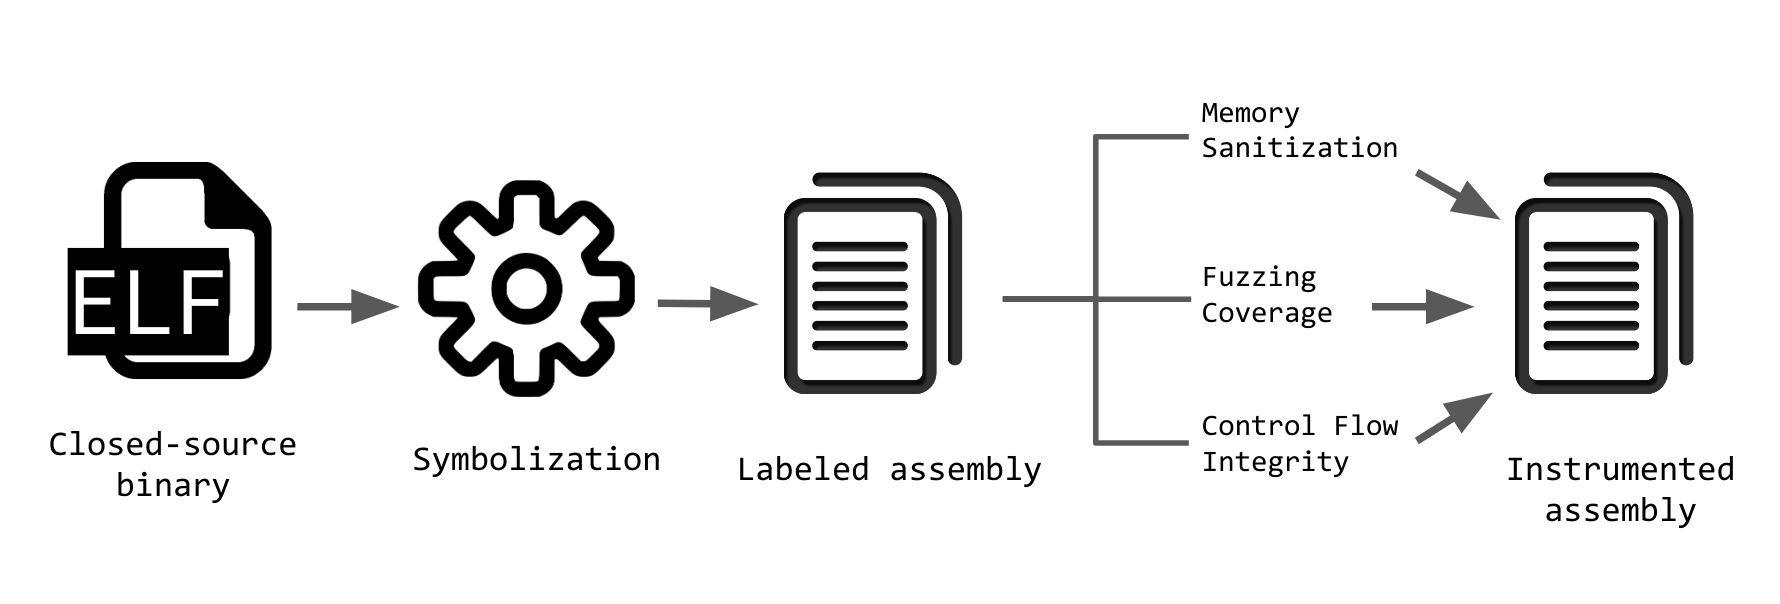
\includegraphics[width=15cm]{symbolizer.png}
\caption{Overview of the structure of \sysname}
\end{figure}

\sysname follows the same structure as \sysnameold and is divided into two main
components: the symbolizer and the instrumentation.  The symbolizer takes care
of loading and analyzing a binary, but its main job is substituting every
reference in the target with assembly labels, plus some minor tasks to keep the
original functionality of the binary intact. 
Listing~\ref{diffass}  shows the output of the symbolization process on a
small example assembly snippet.

One or more instrumentation passes can be enabled to apply 
transformations to the resulting binary. For now, only a single pass is 
implemented (BASan), but many more can be easily added.





\subsection{Differences with \sysnameold}

\sysname uses the same approach for the parsing of the executables, although
with different implementation details to support the \texttt{ARM} architecture (e.g., relocations). The technique to differentiate between references and scalars introduced in \sysnameold is also the same. 

Since this document focuses on the new challenges that the \texttt{ARM} architecture introduced, we will not go into details about the above algorithms, and point the reader to the original \sysnameold paper~\cite{dinesh20oakland} for further reference. 

The novelty in \sysname relies in the additional static analysis methods that we had to develop to support detection of pointer constructions and jump tables. To the best of our knowledge, our work is the first attempt to generate symbolized enlarged jump tables and symbolized pointer constructions. In the next section we will go into detail about the above challenges and how did we solve them.


\section{Key Issues}
The outstanding challenges of statically analyzing and instrumenting ARM 
binaries can be summarized as follows:

\begin{itemize}
	\item Detecting and fixing pointer constructions.
	\item Detecting and symbolizing jump tables.
	\item Supporting extensive instrumentation by enlarging jump tables.  
\end{itemize}

In the following pages we will get into detail for each one of those issues, 
and explain the reasoning behind our solution.

\subsection{Pointer construction}
The Aarch64 instruction set is defined as \emph{fixed size}, because every 
instruction is large exactly 4 bytes. This makes the CPU design simpler,
helps keeping memory always aligned, and permits the CPU to fetch multiple 
instructions at once, since decoding is not necessary to determine instruction 
boundaries. However, despite the many advantages of this characteristic, there 
are some drawbacks too, including not being able to store a pointer in a single 
instruction (as pointers have a size of 8 bytes). The Aarch64 ISA provides two 
main solutions to this problem. 

The first one consists in storing the pointers in a special read-only region of 
memory, called a \emph{literal pool}, and then load those pointers into a 
registers using the special construct \texttt{ldr <reg>, =pointer}, a 
pseudo-instruction that the assembler will translate with the correct memory 
address once \texttt{pointer} has been stored in a literal pool.  Since all 
\emph{ldr} instructions are PC-relative, and since there are 21 bits available 
to store the offset from the PC, the assembler will store \emph{pointer} in a 
literal pool which is in the $\pm$ 1MB range of the \texttt{ldr} instruction.  
While this is a simple and straightforward approach, very useful in the case of 
hand-written assembly, this requires an additional memory access that may 
impact performance in the long run. Furthermore, the assembly will fail if it 
is not possible to store a literal pool in the given range, such as in the case 
of a function larger than 2MB.\@ In that case, it is up to the programmer to 
find a suitable spot for the literal pool, by manually specifying its location 
with the \texttt{.ltorg} assembly directive. It is often recommended to store 
literal pools directly after non-conditional jumps to avoid executing 
them~\cite{literalpools}.

The second solution is to build pointers using multiple instructions and basic 
arithmetic primitives. Aarch64 provides instructions such as \texttt{adrp 
<reg>, pointer}, which loads the base page of a pointer into a register. It is 
a PC-relative instruction, and targets pointers in the $\pm$ 4GB range.  In 
other words, the \texttt{adrp} instruction can point only to memory locations 
that are 4KB aligned. Usually the instruction can be followed by an 
\texttt{add}, a \texttt{sub} or an offset-based load such as \texttt{ldr 
<register>, [<base\_page>, offset]}. This second way, while more contrived and 
certainly harder to read, is faster than the first one as it does not require a 
memory access, and also often benefits from custom hardware optimizations (such 
as in the Cortex A72, one of the most common ARM 
CPUs~\cite{pointeroptimizations}). 

\subsubsection{The global variable problem}
For the reasons stated above, compilers generally use the second option, 
preferring performance over assembly readability. Having each pointer value 
separated in two different instructions makes the static analysis of a binary 
substantially harder. Furthermore, compiler optimizations frequently exacerbate 
the problem, by reusing parts of some pointer values to build new ones, or 
reordering instructions around in such a way that a pointer can be built on two 
instructions which are kilobytes away from each other. In some extreme cases, 
by enabling the \texttt{-O3} optimizations, we found instances of pointers 
built on two instructions that were on different functions, due to the compiler 
optimizing a macro in the C source code. 

An important factor to note is that this behaviours happens exclusively when 
accessing \emph{global variables}, since all code pointers and local variables 
are reachable through a single pc-relative instruction. 

In the symbolization process (that will be explained in detail later), we need 
to know the value of every pointer used in the program, in order to correct it 
when we will add instrumentation later on. Thus we are required to develop an 
analysis technique that lets us recover the value of every single global 
pointer used in the binary. We will now shortly describe the ideas behind the 
solution we implemented.

\subsubsection{Our solution for the global variable problem}

At first, some basic static analysis is performed on the binary, in order to 
recover functions, control flow, basic blocks and disassembly of the 
\texttt{.text} section. After this, we scan the disassembly for each possible 
instance of pointer building in the binary. After analyzing common compiler 
patterns, we found out that the \texttt{adrp} instruction (which loads the base 
page address of a pointer) is an indicator of a possible start of a pointer 
building process. 

After collecting all the possible instances of pointer building, the next step 
is to find out the final pointer value of each one. This turned out to be an 
extremely difficult task, as we soon found out that there are infinitely many 
ways of how a pointer can be built. We implemented a pattern-matching solution 
at first, trying to detect common compiler patterns for pointer building; while 
we correctly found out the value of the vast majority of pointers, a single 
mistake could make the binary crash, and our solution was not working on 
binaries of large sizes, as we inevitably failed to parse at least one or two 
edge-cases.

We later shifted to a different approach: instead of trying to find exact value 
of a pointer by pattern matching, we take the set of all possible values a 
pointer could have and exclude wrong values until possible. Over 90\% of the 
times, this approach leaves only a single value. The rest of the times, only 
two or three values remain, for which we use the old pattern-matching solution 
to understand which of those is the correct one. 

This final solution scales really well, as proved by the fact that we rewrote 
very large binaries and successfully ran them through long benchmarks. For more 
details on how the exclusion algorithm works, see the next chapter, 
Implementation.  


\subsection{Jump table target recovery}
There is a big difference in how jump tables in ARM are implemented compared to 
\texttt{x86}. In fact, in \texttt{x86}, a jump table is represented through a 
list of code pointers in the \texttt{.rodata} section. The assembly generated 
by the compiler will simply load the pointer from the list indexed by the 
number of the case that is going to be executed. 

On ARM, things are different: jump tables are stored as a list of 
\emph{offsets} from the base case (case number 0) in memory. The compiler 
generates assembly that fetches the correct offset based on the case number 
from the list in memory, adds the offset to the base case, and jumps to the 
resulting value. Listing~\ref{lst:jmptbl} shows an example of jump table access 
in \texttt{aarch64}. The first two instructions build a global pointer to where 
the jump table is stored in memory. In line 3 the offset to the corresponding 
case is loaded into register \texttt{w1}, and then later added to the base case 
\texttt{x0} on line 5. 


\begin{lstlisting}[float,floatplacement=H,label={lst:jmptbl},caption={Example of a jump table in \texttt{aarch64}},numbers=left]
adrp x0, <jump_table_page_address>
add x0, x0, <jump_table_page_offset>
ldrb w1, [x0, w1, uxtw]
adr x0, <base case address>
add x0, x0, w1, sxtb 2
br x0
\end{lstlisting}

Furthermore, jump tables in \texttt{aarch64} are complicated by the fact that 
they are often \emph{compressed} in memory. Since they store offsets, not 
pointers, and commonly jump table cases are very close to the base case, 
compilers usually avoid using the full 8 bytes of memory for each case (which 
would be normal in \texttt{x86}), but will use less if possible. For instance, 
if all offsets are less than 256, the compiler will use a single byte in memory 
to store each case.  

\subsubsection{Detection of jump tables}
The first problem we had to face was the discovery of jump tables. While they 
have a very distinct pattern (a load from memory, followed by some arithmetic, 
and then an indirect jump), many other constructs share similar patterns (like 
using a callback in a struct). We found out that a reliable way of detecting 
them is by backward-slicing every time the disassembler encountered an indirect 
jump, and then verifying if the value of the register used for the indirect 
jump could be represented with an expression which could be resolved statically 
and matched a very defined pattern (load 1/2/4 bytes from memory, load a base 
address, add the offset and then jump to the result). 

To represent the value of a register as an expression, we developed a simple
pseudo-emulation engine that steps backwards from a given instruction, 
following control flow and building step by step the resulting expression, 
similar to what a dumbed-down symbolic executor would output. The 
pseudo-emulation engine is limited, supports circa 20 instructions, as 
emulating ARM was out of the scope of the project and we only needed it for 
jump table detection. A detailed explanation of how it works can be found in 
the next chapter.

\subsubsection{Detection of jump tables size}
Another problem that quickly arose from the peculiarities of ARM jump tables is 
that it is much harder to estimate the number of cases that a jump table 
supports, compared to \texttt{x86}. In fact, in \texttt{x86}, simple heuristics 
such as scanning memory for contiguous sections of valid instruction pointers 
until an invalid one is found can go a long way. However, as stated before, in 
ARM jump tables are indistinguishable from random bytes, so it is impossible to 
use heuristics to understand the bounds of a particular jump table in memory.

We found that backward slicing is again a robust solution here too. After 
detecting a jump table, we can identify the instruction that takes care of 
loading the offset from memory, and from there we mark the register that holds 
the value of the number of the case that is going to be executed.  
Backward-slicing until a comparison operation is performed on the marked 
register, bounding the number of cases to an absolute number, turned out to be 
a very reliable solution.  

\subsection{Enlarging jump tables}
Another problem spawned from how jump tables are represented in ARM comes up 
when instrumenting a function that contains a jump table. In fact, it is very 
likely that adding too much instrumentation inside a single case could 
\emph{overflow} one of the offsets that stored its distance from the base case.
Especially when maximum compression is used and offsets are stored in a single 
byte, it is very common to overflow multiple of them even with light 
instrumentation. 

This was one of the harder problems to fix, and we considered the following 
solutions:
\begin{itemize}
	\item Expand the jump table in memory. Enlarge the \texttt{.rodata} section 
		and move everything to make space in memory for the expanded jump 
		table. While possible, this would have been be a drastic change that 
		was not scalable or easily implemented.
	\item Create a new jump table in a new section, and patch the pointer 
		building code at the start of the jump table access code. While this 
		was the easiest solution to implement, we discarded it because of the 
		additional space required and its poor scalability.
	\item Divide all the offsets by the same constant value. Normally, all 
		offsets of a jump table represent the distance between a case and the 
		base case expressed in bytes divided by 4. This is because each 
		instruction is 4 bytes long, and it would not make sense to point 
		inside an instruction. In fact, in Listing~\ref{lst:jmptbl}, line 5, we 
		can see how the offset is shifted by 2 to the left (so multiplied by 
		4). This is automatically done by the compiler. However, we can use the 
		same technique the compiler uses and store offsets divided by 8, 16 or 
		more, and changing how much the offset is shifted to the left before 
		being used, thus enabling us to store larger differences in a single 
		byte. 

		The trade-off with this approach is that offsets can no longer point to 
		a single instruction, but to a block of 2, 4 or more instructions, 
		depending on how much enlargement was needed. To make sure that each 
		offset points to the right instruction, some light \emph{nop-padding} 
		is applied between cases to make sure that alignment is correct every 
		time.
\end{itemize}

We ended up using the last solution, as even if it was slightly more complex to 
implement, it would help us keep the original memory layout of the binary, 
which is a very desirable property in binary rewriting. 

\subsection{Control Flow broken by instrumentation}
When adding substantial amount of instrumentation to a binary, some pc-relative 
branches can break, like the instruction \texttt{cbz}, which cannot jump to 
addresses farther than 1MB\@. 

In this cases we fix the relevant instruction by making them point to a some 
additional instrumentation containing a trampoline to the original target of 
the branch. 




\subsection{Instrumentation register saving}

We designed \sysname to support any kind of instrumentation, without 
sacrificing performance and functionality. We realized though that many 
different kinds of instrumentation require some intermediate calculations to be 
saved in registers. This was causing noticeable overhead in the 
instrumentation, as registers needed to be saved on the stack and restore in 
every instrumented location. 

To avoid this additional overhead, we implemented a static analysis of register 
usage for every function, with instruction-level granularity (i.e., the result 
of the analysis is the set of registers that can be freely used without saving 
them for every instruction inside a given function). The instrumentation can 
then use the set of free registers without worrying about hindering the 
original functionality of the binary. 



%%%%%%%%%%%%%%%%%%%%%%%%
\chapter{Implementation}
%%%%%%%%%%%%%%%%%%%%%%%%
%The implementation covers some of the implementation details of your project.
%This is not intended to be a low level description of every line of code that
%you wrote but covers the implementation aspects of the projects.

%This section is usually 3-5 pages.

In this chapter we cover the implementation of the rewriter, and of bASAN, the memory
sanitization instrumentation pass. We will also share details on the optimizations
we implemented to minimize instrumentation overhead.

\section{Symbolizer}


Symbolization requires detection of every single pointer and control flow
mechanism in the binary. In \texttt{aarch64}, this may prove to be harder than
it looks, as in fact pointer construction patterns are difficult to recover
and jump tables are not as friendly as they are in x86. 
In the following subsections we will go over each problem and explain our
approach to tackle it. 



\subsection{Pointer Construction}

\subsubsection{Detection and recovery of pointers}

Standard compilers (clang, gcc) that target \texttt{aarch64} use a common 
pattern for building pointers: an \texttt{adrp} instruction, loading the page 
of the destination address, and then either an \texttt{add} or similar arithmetic 
instruction to fix the offset inside the page, or a memory operation like 
\texttt{ldr} or \texttt{str} that include the offset inside the page 
(e.g., \texttt{ldr x0, [x1, 256]}).

We implemented two different approaches and combined them together to 
successfully recover pointers in \texttt{aarch64} binaries.
The first one is based on pattern matching. We first build a list of 
possible pointer building locations, enumerating all instances of the \texttt{adrp} 
instruction. Next, we tried to find all \texttt{add}, \texttt{ldr}, or 
\texttt{str} instructions (or their variants) that used the register that was 
partially built with the \texttt{adrp}, and tried to recover the original
pointer by emulating the arithmetics involved in those instructions.
This approach alone was not enough because of the following 
difficulties:

\begin{itemize}
	\item Multiple pointers built with the same \texttt{adrp}:
		\autoref{pointers} shows how sometimes the same \texttt{adrp} page
		loading instruction is used for multiple pointer constructions,
		sometimes very far away from each other
	\item Moving base page register: another difficulty was that sometimes the 
		register used to store the base page changed in the middle of the 
		pointer construction, like in \autoref{pointers2}
	\item Base register stack saving: in very large functions, sometimes the 
		base registers were loaded at the start and saved on the stack, to be 
		later restored and used for pointer building. An example is present in 
		\autoref{pointers3}
\end{itemize}

\begin{lstlisting}[float,floatplacement=H,label=pointers,caption={Example of multiple pointers built from the same \texttt{adrp} instruction}]
adrp x0, 0xab0000
add  x1, x0, 256   ; pointer 0xab100
ldr  x2, [x0, 512] // pointer 0xab200
add  x0, x0, 128   // pointer 0xab080
\end{lstlisting}
\begin{lstlisting}[float,floatplacement=H,label=pointers2,caption={Example of changing register during
pointer construction}]
adrp x0, 0xab0000
mov  x1, x0
add  x1, x1, 256   // pointer 0xab100
\end{lstlisting}
\begin{lstlisting}[float,floatplacement=H,label=pointers3,caption={Example of base page register stack
saving}]
adrp x0, 0xab0000
str  x0, [sp, -16!]
...
ldr  x3, [sp, 16!]
add  x3, x3, 512   // pointer 0xab200
\end{lstlisting}


We implemented a light data flow recovery algorithm
that statically analyzed the control flow and the stack usage of a given
function, following around the register used for the \texttt{adrp} and checking
for its usage, to address all the difficulties stated above. However, it is
particularly hard to support every single edge case, and missing a single
pointer symbolization is fatal and will cause a crash when the pointer is 
dereferenced (which sometimes happens a while after the pointer is built, 
and can be very time consuming to detect and debug). 
While this pattern matching approach alone worked with the vast majority of
pointer construction, it was insufficient to completely symbolize all pointers
and failed on large binaries. 

Our second approach took advantage of the fact that \sysname does not 
instrument data sections, and the vast majority of global variables point to
those. Instead of trying to parse the pointer building patterns, we try to
guess which section of the original binary an \texttt{adrp} could be pointing
to. Since the \texttt{adrp} loads a base page, and a page offset is added, the
sections that can be addressed by a single pointer constructions are those that
overlap the \texttt{adrp} address $\pm$ 1 KB.\@ Since all sections except
\texttt{.text} are not instrumented, if we are able to narrow down the possible
target of a pointer construction to a single section, we can symbolize the
pointer by just adjusting the starting 
\texttt{adrp} to correctly address the same symbolized section as in the 
original binary, since offsets used by \texttt{add} or \texttt{ldr} will stay 
the same.
For example, if we encounter the instruction \texttt{adrp x0, 0xab000} and the
only section close enough is the \texttt{.bss} that starts at address
\texttt{0xab256}, we can symbolize every pointer construction on \texttt{x0} by
changing the above \texttt{adrp} to \texttt{ldr x0, =(.bss - 256)}.



This second approach is more stable, as it does not
incur in any of the problems stated above. However, it was not always
applicable, as especially in smaller binaries multiple sections could be in the
$\pm$ 1 KB range from the \texttt{adrp} destination address; in that case, we
used some simple data flow analysis to exclude as many sections as possible.
We found out that in around 99\% of cases we are able to use this \texttt{adrp}-adjusting
approach without needing to do any heuristics at all. In the case we are not able
to determine which single section the \texttt{adrp} is pointing to, we fall back
to the first pattern matching based approach. 


\subsection{Symbolization of pointers}

After detection of a pointer construction in the target binary, it is still not 
trivial how to symbolize a pointer. There are two solutions to this problem: 
using \emph{literal pools} and using pointer construction.

\subsubsection{Literal pools}

A literal pools is a special region of memory in a binary that stores absolute
addresses. It is widely used in \texttt{ARM} to overcome the challenge of not
being able to store a pointer in a single instruction. 

The \texttt{ARM} assembly specification~\cite{literalpoolsarm} states that the
assembler will store a pointer in a literal pool when using the following
construct: \texttt{ldr x0, =<pointer>}.  The \texttt{=<pointer>} part will be
assembled with a pc-relative load to the nearest literal pool that contains the
full pointer address.  The location of the literal pool must be manually
specified in assembly through the \texttt{.ltorg} directive. Usually, literal
pools are stored between functions in the \texttt{.text} sections. Since the
pc-relative load can only target addresses in the $\pm$ 1 MB range, literal
pools must be stored inside functions if they are larger than 2 MB. 

In our first implementation we used literal pools to symbolize pointers, but we
detected noticeable overhead introduced even without instrumentation added. The
runtime of binaries without instrumentation was around 5\% higher when compared
to the original binaries.  The reason behind the additional overhead is
twofold: first, each pointer retrieved through literal pools requires a memory
access each time; secondly, literal pools occupy precious space in the
\texttt{.text} section causing more cache misses than necessary. 


\subsubsection{Pointer construction symbolization}

To avoid the overhead introduced by the usage of literal pools, we decided to
use pointer construction ourselves. The symbolization of a pointer construction
is composed of two parts: the symbolized \texttt{adrp} base page loading and
the symbolized \texttt{add} for the page offset. An example of such process can
be found in Listing \ref{lst:construction}. The \texttt{adrp} is symbolized by just
substituting its argument with the symbolized counter part.  The page offset part,
instead, is symbolized through a special assembler directive that evaluates to the
last 12 bits of the specified assembly label (and 12 bits are enough to specify
the offset inside a page). 

\begin{figure}[h]
\label{lst:construction}
\begin{minipage}{\textwidth}
\begin{lstlisting}[]
0x400: adrp  x0, 0xab000
0x404: add x0, x0, 256              // pointer to 0xab100
\end{lstlisting}
\end{minipage}

\begin{minipage}{\textwidth}
	\begin{lstlisting}[]
.LC400: adrp  x0, .LCab100          // base page 
.LC404: add x0, x0, :lo12:.LCab100  // page offset
\end{lstlisting}
\end{minipage}
	\captionof{lstlisting}{Example pointer construction in the original binary
	(above) and symbolized pointer construction (below)}
\end{figure}



\section{Jump Tables}

Switch statements in \texttt{ARM} binaries are stored as a table of offsets,
instead of absolute addresses like in \texttt{x86}. This makes symbolizing them
particularly tricky. First of all, detecting them is not easy. Listing
\ref{omgjmptbl}shows how they do not have a particular pattern in memory. In
this section we will go over what was our approach to finding them and how did
we symbolize them without breaking their functionality.



\begin{figure}[h]
\centerfloat
\begin{minipage}{.60\textwidth}
\begin{lstlisting}[numbers=none]
0x400: adrp x0, 0x8000
0x404: add x0, x0, 3
0x408: ldrb w1, [x0, w1, uxtw]
0x40c: adr x0, 0x418
0x410: add x0, x0, w1, sxtb 2
0x414: br x0
0x418: movz x0, 1   // case 0,1,2
0x41c: ret
0x420: movz x0, 10  // case 3
0x424: ret
0x428: movz x0, 100 // case 4
0x42c: ret
\end{lstlisting}
\end{minipage}\hspace{1cm}
\begin{minipage}{.50\textwidth}
\begin{lstlisting}[numbers=none]
0x8003: byte 0x0   // case 0
0x8004: byte 0x0   // case 1
0x8005: byte 0x0   // case 2
0x8006: byte 0x8   // case 3
0x8007: byte 0x10  // case 4
\end{lstlisting}
\end{minipage}
\captionof{lstlisting}{Left: code for a performing a switch. Register w1
	holds the case number that is going to be executed. The offset is loaded at
	\texttt{0x408}, which is added to the base case address (loaded at
	\texttt{0x40c}) and then jumped into (\texttt{0x414}). \\ Right:
	corresponding jump table in memory, with 5 cases each occupying a single
	byte in memory. Cases can be repeated, and are impossible to distinguish
	from other data in memory.}
\label{omgjmptbl}
\end{figure}



\subsection{Detection of jump tables}
Unlike \texttt{x86}, on \texttt{ARM} jump tables are not encoded as sets of code
pointers in the \texttt{.rodata} section.
Similar to \texttt{x86}, on \texttt{ARM} compilers use specific patterns to construct
code pointers, for example through
\autoref{jmptbl} and \autoref{omgjmptbl}. 
Our algorithm to detect a jump table pattern works as follows:

\begin{itemize}
	\item Recover the complete control flow of each function, using the linear sweep technique.
	\item Mark all indirect jump locations, identified by \texttt{br} instructions.
	\item Backwards-slice the code to find all paths that may lead to
		this instruction, with a maximum path length of 50 instructions. This upper bound is generous (in all the cases we analyzed 15 instructions were enough) and prevents computationally expensive path explosions.
	\item Reverse-emulate every path, and store every possible (symbolized)
		value that the register of the indirect call can have.
	\item If the value that the register can have is the same for every path,
		and corresponds to a jump table symbolic expression, then mark the
		\texttt{br} instruction as part of a jump table construct.
\end{itemize}

To reverse-emulate every path that leads to the indirect call, we implemented a
very limited \texttt{aarch64} symbolic instruction emulator. It supports around
20 ARM instructions (all those that are common in jump table constructs, plus
arithmetic instructions and a few memory-related ones).  A very simple example of the
output of this emulator can be found in \autoref{emulator} (jump table constructs are 
often more nuanced and interleaved with other instructions).

After we get the symbolic value of the indirect jump register, we compare it to
the standard jump table expression, which is the following:

\texttt{base\_case\_addr + (*(jump\_table\_base\_addr + (register\_case\_number * ?)) \textless\.\textless\  ?)} 

The symbol \texttt{?} is a wildcard for any (positive) integer value.
\texttt{base\_case\_addr} is the address of case 0 in the jump table.
\texttt{jump\_table\_base\_addr} is instead the address in memory of the jump
table offsets. Finally, \texttt{register\_case\_number} is a register with as
value the number of the case that is going to be executed. 

Finally, if the indirect call is recognized as a jump table, the last step is
determining how many cases the switch represented by the jump table is made of.
We solved this by backward-slicing from the instruction loading the case number
(\texttt{0x408} in \autoref{emulator}) and looking for an upper-bound
comparison with a constant value on the register that holds the current case
number to be executed (\texttt{w1}).  If the comparison is directly followed by
a jump, than we mark the jump target location as the ``default'' case and set
the number of cases of the jump table based on the constant of the comparison.


\begin{figure}[h]
\begin{lstlisting}[numbers=none]
0x3f8: cmp w1, 128
0x3fc: b.hi .default_case
0x400: adrp x0, 0x8000
0x404: add x0, x0, 3
0x408: ldrb w1, [x0, w1, uxtw]
0x40c: adr x0, 0x418
0x410: add x0, x0, w1, sxtb 2
0x414: br x0
\end{lstlisting}
\begin{lstlisting}[numbers=none]
Analyzing 0x414: br x0
x0 = x0
x0 = x0 + (w1 << 2)
x0 = 0x418 + (w1 << 2)
x0 = 0x418 + (*(x0 + w1*1) << 2)
x0 = 0x418 + (*(0x8003 + w1*1) << 2)
Result:
Base case: 0x418
Jump table addr: 0x8003
Case number reg: w1
Number of cases: 128
Shift: 2
\end{lstlisting}
\captionof{lstlisting}{Above: example of a jump table pattern. Below: output of
our symbolic emulator. }
\label{emulator}
\end{figure}


\subsection{Jump Table symbolization}

The symbolization of a jump table in memory is done using the assembler's 
support for simple arithmetic on assembly labels. Since on ARM a jump table
is no more than a sequence of offsets from a base instruction, we symbolize
that with differences between assembly label. An example of this can be seen
in \autoref{omgjmptbl}.

Since the offsets in the symbolized version are calculated with assembly labels,
any amount of code can be added between cases, and the assembler will make sure
that the jump table will work correctly. This is one of the cases where the benefits
of using symbolization as a rewriting technique really shines, as it gives us the 
freedom of inserting arbitrary instrumentation (even by hand) without having to worry
about correcting references.

However, there is a catch: adding \emph{too much} instrumentation could
overflow the value used to store the offset from the base case. In the example
in \autoref{omgjmptbl}, if there are more than 256 instructions between a case
and the base case, the offset will overflow as it is stored in a single byte.
In the next subsection we will cover how we actually support adding arbitrary
amount of instrumentation. 

\begin{figure}[h]
\centerfloat
\begin{minipage}{.55\textwidth}
\begin{lstlisting}[numbers=none]
0x8003: byte 0x0   // case 0
0x8004: byte 0x0   // case 1
0x8005: byte 0x0   // case 2
0x8006: byte 0x8   // case 3
0x8007: byte 0x10  // case 4
\end{lstlisting}
\end{minipage}\hspace{1cm}
\begin{minipage}{.59\textwidth}
\begin{lstlisting}[numbers=none]
0x8003: byte (.LC418 - .LC418) / 4
0x8004: byte (.LC418 - .LC418) / 4
0x8005: byte (.LC418 - .LC418) / 4
0x8006: byte (.LC420 - .LC418) / 4
0x8007: byte (.LC428 - .LC418) / 4
\end{lstlisting}
\end{minipage} 
\captionof{lstlisting}{Left: jump table as stored in memory as
found in the original binary. Right: symbolized jump table in the output of
\sysname.}
\label{omgjmptbl}
\end{figure}


\subsection{Jump Table enlargement}

When too much instrumentation between jump table cases is added, the value used
to store the offset from the base case can overflow. To address this, we
implemented support for using a larger divisor when storing assembly label
differences.  As an example, instead of storing \texttt{(LC418 - .LC410) / 4}
like in \autoref{omgjmptbl}, we can store \texttt{(.LC418 - .LC410) / 8} to fit
up to 512 instructions between \texttt{.LC418} and \texttt{.LC410}. The same reasoning
can be reapplied with higher powers of two. 

However, using a divisor higher than 4 means losing precision in the possible
addresses of the cases we want to represent. Since 4 bytes is the size of each
instruction, dividing by 4 means that every instruction can be targeted;
dividing by 8 means that only one every two instructions can be targeted. To
avoid losing precision over which instruction can be targeted or not, we insert
\texttt{nop} padding before each case of the jump table in the output assembly
in order to make every case targetable by an offset, with the amount of nops
depending on how high is the divisor (e.g., dividing by 8 means that each case
must by 8-byte aligned, so using up to 1 nop before each case; dividing by 16
means using up to 3 nops, and so on). Since the number of nops inserted depends on 
alignment, we leave this task to the assembler using the \texttt{.align} directives.

After changing the divisor, we also need to change the indirect jump calculations in the
binary's code to match the new shift value. Usually, the offset to be added is multiplied by
4 using an instruction like \texttt{add x0, x0, w1, sxtb 2} (which shifts left by 2), as
can be seen in \autoref{emulator}. We change the shift value according to how high we set
the dividend in the symbolized jump table (the \texttt{add} instruction support shifting left
up to 4, but we insert a standard \texttt{lsl} instruction before if it's higher than 4). 

An example of this can be found in Listing \ref{enlarged}.

\begin{figure}[h]
\begin{lstlisting}[numbers=none]
.LC400: adrp x0, .LC8003
.LC404: add x0, x0, :lo12:.LC8003
.LC408: ldrb w1, [x0, w1, uxtw]
.LC40c: adr x0, .LC418
.LC410: add x0, x0, w1, sxtb 4
.LC414: br x0
.align 4
.LC418: movz x0, 1 // case 0,1,2
.LC41c: ret
.align 4
.LC420: movz x0, 10 // case 3
.LC424: ret
.align 4
.LC428: movz x0, 100 // case 4
.LC42c: ret
...
...
0x8003: byte (.LC418 - .LC418) / 16
0x8004: byte (.LC418 - .LC418) / 16
0x8005: byte (.LC418 - .LC418) / 16
0x8006: byte (.LC420 - .LC418) / 16
0x8007: byte (.LC428 - .LC418) / 16
\end{lstlisting}
\captionof{lstlisting}{Example of enlarged symbolized jump table. The shift value at \texttt{0x410} is increased from 2 to 4, and the divisor at \texttt{0x8003} is increased from 4 to 16. Before each case, an \texttt{.align 4} assembly directive is inserted, as each of them need to be aligned to 16 bytes.}
\label{enlarged}
\end{figure}


\section{Instrumentation (BASan)}
The ASan instrumentation was designed to be compatible with the 
AddressSanitizer libraries provided by Google, \texttt{libasan}. We carefully 
selected shadow memory offsets and sizes to match those included in 
\texttt{libasan}.  The library will hook on each call to \texttt{malloc} and 
\texttt{free}, writing in the shadow memory the available bytes that can be 
used. \sysname takes care of finding each access in memory and inserting 
instrumentation just before each access to check the relevant bytes of shadow 
memory and error out in case an overflow or other memory corruption was found.


\begin{lstlisting}[float,floatplacement=H,language=C,label={lst:asan},caption={AddressSanitizer checking algorithm example implementation}]
byte shadow_value = *(MemToShadow(address));
if (shadow_value) {
  if ((address & 7) + AccessSize - 1 >= shadow_value) {
	ReportError(address, AccessSize);
  }
}
\end{lstlisting}

Listing~\ref{lst:asan} shows the ASan checking algorithm in high level. To 
implement it as an instrumentation pass, we manually wrote assembly code that 
matched its functionality and could be adapted to both reads and stores.  
Different versions of ASan snippets were developed depending on the size of the 
store/load, to ensure maximum efficiency and avoid wasting calculations at 
runtime. An example of an instrumented instruction can be found in the listing 
below:

\todo{Add comparison between non-instrumented and instrumented 8-byte load (the 
simplest case)}

Unfortunately, the BASan instrumentation pass is not completely equivalent to 
its source based counterpart, in fact we can highlight the following 
differences:
\begin{itemize}
	\item Missing global variable bounds checking: without the source code, it 
		is impossible to distinguish boundaries between global variables in 
		data section. For this reason, checks on global variables are disabled.
	\item Missing stack variables bounds checking: similar to above, without 
		source code it is extremely hard to find boundaries between variables 
		on the stack.
	\item Number of instrumented locations: ASan used as a compiler pass is 
		able to prune the checking on a lot of memory accesses, since on many 
		instances the safeness of a memory access can be determined at 
		compile-time with the source code at hand. However, \sysname works only 
		on binaries and thus is forced to instrument all memory accesses.
\end{itemize}
Despite the following limitations, the BASan instrumentation pass provides the 
same core functionality of the original ASan compiler pass (memory sanitization 
on the heap), and with very little additional overhead.

\subsubsection{Optimization: register savings}
The snippets of assembly used to implement ASan memory checking require some 
temporary register usage to store intermediate calculations, and thus require 
special precautions before inserting them in the middle of a binary. Our first 
approach was to save the values of each register we were planning to use on the 
stack, and then restore the old values as the last step of the instrumentation.  
However, we quickly realized that those frequent memory accesses were 
introducing noticeable overhead. 

We then switched to performing a static analysis of register usage on every 
function of the binary, in such a way that at any given instruction we know 
which registers can be freely used and which cannot be modified without 
hindering the correct execution of the binary. Then, when inserting the 
instrumentation, we modify the snippets in such a way that they will try to use 
as many `free' registers as possible, while saving the others on the stack.

Of particular note is the saving of the value of register \texttt{ncvz}, which 
holds the condition flags in \texttt{aarch64}. This register is always saved 
and restored at each instrumented location, as all ASan snippets contain a 
conditional branch for the error checking. 

\todo{If needed, put other optimizations here, like batching}


%%%%%%%%%%%%%%%%%%%%
\chapter{Evaluation}
%%%%%%%%%%%%%%%%%%%%


In this section we validate the claims that we made earlier by performing experiments.
We show that \sysname can symbolize and instrument ARM binaries with the performance of
source based instrumentation without compromises on its scalability.

\section{Setup and Hardware} 
We decided to run experiments on two different setups. The first is a low end system, while
the second one is a very high end configuration, in order to highlight the differences between
the two device classes. 
The machines we had available are the following:
\begin{itemize}
	\item A raspberry Pi 4B, with a Cortex A-72 (1.5GHz) CPU and 4GB of RAM
	\item An Atlas/A57 (2.4GHz) CPU with 64 GB of RAM
\end{itemize}

%\mat{Why use two machines? A low end and a high end configuration to highlight the two different
%device classes.}

To benchmark the performance of rewritten binaries, we used the SPEC CPU 2017
benchmark suite~\cite{speccpu2017}.  We used only the C language benchmarks as
\sysname does not (yet) support the symbolization of C++ exceptions. The list of the
benchmarks can be seen in \autoref{tabularasa}.  All of the benchmarks were run on
both machines, but on the raspberry some benchmarks were excluded from the results
as 4GB of RAM were not enough to avoid using swap memory, compromising the
experiments. The Atlas machine was generously hosted by the
CloudLab project~\cite{cloudlab} in their Utah data center. 

The benchmarks were compiled with the gcc compiler version 7.5.0 on Ubuntu
18.04. The following command line flags were used to compile the baseline
benchmark binaries: \texttt{-O3 -fgnu89-inline -fno-strict-aliasing}, in
addition to the flags to produce position independent executables. 
The \texttt{-fgnu89-inline} flag uses GNU semantics for inline functions, and
resolves issues with duplicate symbols errors during the compilation of the
\texttt{gcc} benchmark.  The \texttt{-fno-strict-aliasing} flag disables GCC's
aggressive aliasing compilation,and is recommended to be used by the SPEC CPU
manual~\cite{specaliasing} to avoid problems with the \texttt{perlbench}
benchmark. 

To demonstrate the scalability of our approach, we rewrite binaries as large as
the \texttt{gcc} benchmark (> 10MB).  We evaluate the performance of the
symbolization engine by running the benchmarks with the binaries of each
benchmark rewritten by \sysname without adding any kind of instrumentation. We
then evaluate the performance of our memory sanitization instrumentation pass
by comparing it against its source based equivalent
(\texttt{-fsanitize=address} in the compiler flags), and against the equivalent
functionality implemented using a dynamic instrumentation approach, by using
Valgrind with the memory sanitization option (\texttt{valgrind
--tool=memcheck}).


\section{Performance}

%.text size
%imagick_r    -  00000000001d87ec
%lbm_r        -  000000000000290c
%ldecod_r     -  0000000000090494
%mcf_r        -  00000000000078f4
%nab_r        -  000000000002f8c4
%perlbench_r  -  00000000001f96ec
%x264_r       -  0000000000089a7c
%xz_r         -  000000000002731c

% number of functions
%cpugcc_r     -  11799
%imagick_r    -  2187
%lbm_r        -  28
%ldecod_r     -  697
%mcf_r        -  46
%nab_r        -  235
%perlbench_r  -  2408
%x264_r       -  547
%xz_r         -  360


\begin{table}
\centering
\begin{tabular}{lrrrr}
\toprule
	\textbf{Name} & \textbf{Size} & \textbf{Stripped size} &  \textbf{.text size} & \textbf{Functions} \\
\toprule
	\texttt{cpugcc\_r   }              & 63 MB  & 10 MB  & 8912092 & 11799 \\
	\texttt{perlbench\_r} \hspace{2em} & 11 MB  & 2.5 MB & 2070252 & 2408  \\
	\texttt{imagick\_r  }              & 2.4 MB & 2.2 MB & 1935340 & 2187  \\
	\texttt{x264\_r }                  & 687 KB & 645 KB & 563836  & 547   \\
	\texttt{nab\_r      }              & 249 KB & 229 KB & 194756  & 235   \\
	\texttt{xz\_r   }                  & 244 KB & 215 KB & 160540  & 360   \\
	\texttt{mcf\_r      }              & 45 KB  & 38 KB  & 30964   & 46    \\
	\texttt{lbm\_r      }              & 23 KB  & 18 KB  & 10508   & 28    \\
\bottomrule
\end{tabular}
	\caption{Name and size of the SPEC CPU2017 benchmarks written in C. \todo{add basic block number}}
\label{tabularasa}
\end{table}

\subsection{Symbolization performance}

\autoref{plot1} and \autoref{plot2} demonstrate how the overhead of the
symbolization process is very small. Detailed results can be found in
\autoref{labellatabella}.  The average overhead is 0.76\%, in line with other
state of the art static rewriters~\cite{egalito}.  This kind of overhead is
probably due to unoptimal realignment of sections and code, as we produce
position independent assembly without low level optimizations such as cache
hits maximization, leaving this work entirely to the linker. Another important
factor for the overhead is that each pointer building instruction \texttt{adrp}
is symbolized with two instructions (an \texttt{adrp} followed by an
\texttt{add}); so for each global variable access the binary makes the CPU will
lose a clock cycle (probably less, as many ARM CPUs have hardware optimizations
for \texttt{adrp+add} sequences of instructions~\cite{pointeroptimizations}).

Interestingly, at first we used to have substantial overhead from symbolization
alone.  This was on a early stage of the project, where we used literal pools
to symbolize global variable pointer constructions, instead of generating
symbolized pointer constructions ourselves like compilers do, mostly because
using literal pools was simpler to debug and faster to implement.  However,
literal pools introduce an additional instruction (a memory load), plus they
require space in the \texttt{.text} section, reducing cache performance.
\autoref{slowpools} demonstrates how the much overhead decreased when we
switched to symbolized pointer constructions, from an average of 4.12\% to
0.76\%. 

The most affected benchmark by the symbolization overhead is
\texttt{perlbench}, and this fact is consistent with our measurements (as
\texttt{perlbench} has an order of magnitude more global variable accesses
executed compared to the other benchmarks,) and is also the benchmark which
benefited the most from the removal of literal pools.  A negative overhead is
present on the \texttt{mcf} benchmark, but we consider it small enough to lie
inside measurement error. 



\begin{table}

\centerfloat
\sisetup{detect-weight=true}
\sisetup{mode=text}
\robustify\bfseries
	\begin{tabular}{lS[table-format=5]S[table-format=11]S[table-format=1.2]S[table-format=3.2]}
\toprule
		\textbf{Name} \hspace{4em} &
		{\parbox[c]{2.5cm}{\centering\textbf{Static pointer\\constructions}}} &
		{\parbox[c]{3.5cm}{\centering\textbf{Dynamic pointer\\constructions}}} &
		{\textbf{Literal pools}} &
		{\parbox[c]{3.5cm}{\centering\textbf{Symbolized\\pointer building}}} \\
\toprule

		%\texttt{perlbench\_r} & 34285 & 1.6$e^{11}$ & 10.71\si{\percent} & 5.21 \si{\percent} \\
		%\texttt{imagick\_r}   & 19127 & 1.6$e^{10}$ & 1.07 \si{\percent} & 0.33 \si{\percent} \\
		%\texttt{nab\_r      } & 2003  & 2.8$e^{10}$ & 0.00 \si{\percent} & 0.00 \si{\percent} \\
		%\texttt{xz\_r   }     & 1087  & 1.4$e^9$    & 2.39 \si{\percent} & 2.39 \si{\percent} \\
		%\texttt{mcf\_r      } & 108   & 7.9$e^6$    & 2.42 \si{\percent} & 1.20 \si{\percent} \\
		%\texttt{lbm\_r      } & 90    & 3.6$e^5$    & 0.91 \si{\percent} & 1.03 \si{\percent} \\
		%\textbf{Average} &&& \bfseries 3.51\% & \bfseries 1.94\% \\
		% old raspberry results

		\texttt{perlbench\_r} & 34285 & 168797437831& 19.48\si{\percent} & 2.91  \si{\percent} \\
		\texttt{gcc\_r}       & 9095  & 1232266305  & 4.10 \si{\percent} & 0.95  \si{\percent} \\
		\texttt{imagick\_r}   & 19127 & 16275621901 & 1.75 \si{\percent} & 0.30  \si{\percent} \\
		\texttt{nab\_r      } & 2003  & 28193001045 & 0.88 \si{\percent} & 0.34  \si{\percent} \\
		\texttt{xz\_r   }     & 1087  & 1471854761  & 0.33 \si{\percent} & 0.44  \si{\percent} \\
		\texttt{mcf\_r      } & 108   & 7909505     & 1.07 \si{\percent} & -0.07 \si{\percent} \\
		\texttt{lbm\_r      } & 90    & 36160       & 0.08 \si{\percent} & 0.59  \si{\percent} \\
	\midrule
		\textbf{Average} & \text{-} & \hfill\text{-}\hfill & \bfseries 4.12\% & \bfseries 0.76\% \\
\bottomrule
\end{tabular}
\caption{Overhead of \sysname on the Atlas machine without instrumentation
	comparing the recovery of pointers by using literal pools and by using
	symbolized pointer building.  }
\label{slowpools}
\end{table}

\subsection{Memory sanitization performance}


In this section we compare the overhead introduced by \sysname's memory
sanitization instrumentation and the overhead introduced by adding memory
sanitization during compilation (\texttt{-fsanitize=address}).  

An overview of the results can be seen in \autoref{plot1} for the Atlas machine,
and in \autoref{plot2} for the Raspberry. Both figures show the same pattern: 
memory sanitization introduces some overhead but the execution time is still comparable
to source-based instrumentation. However, it can be seen that the Raspberry suffered
from a slightly higher overhead with instrumentation enabled. We think that one of the
possible causes of this is that a low-end system like the Raspberry suffers more from
cache misses than a high-end system (and memory sanitization is a very heavy instrumentation
that increases code size by up to three-fold, substantially degrading cache performance) \todo{are you sure of this??}. 

\begin{figure}[h]
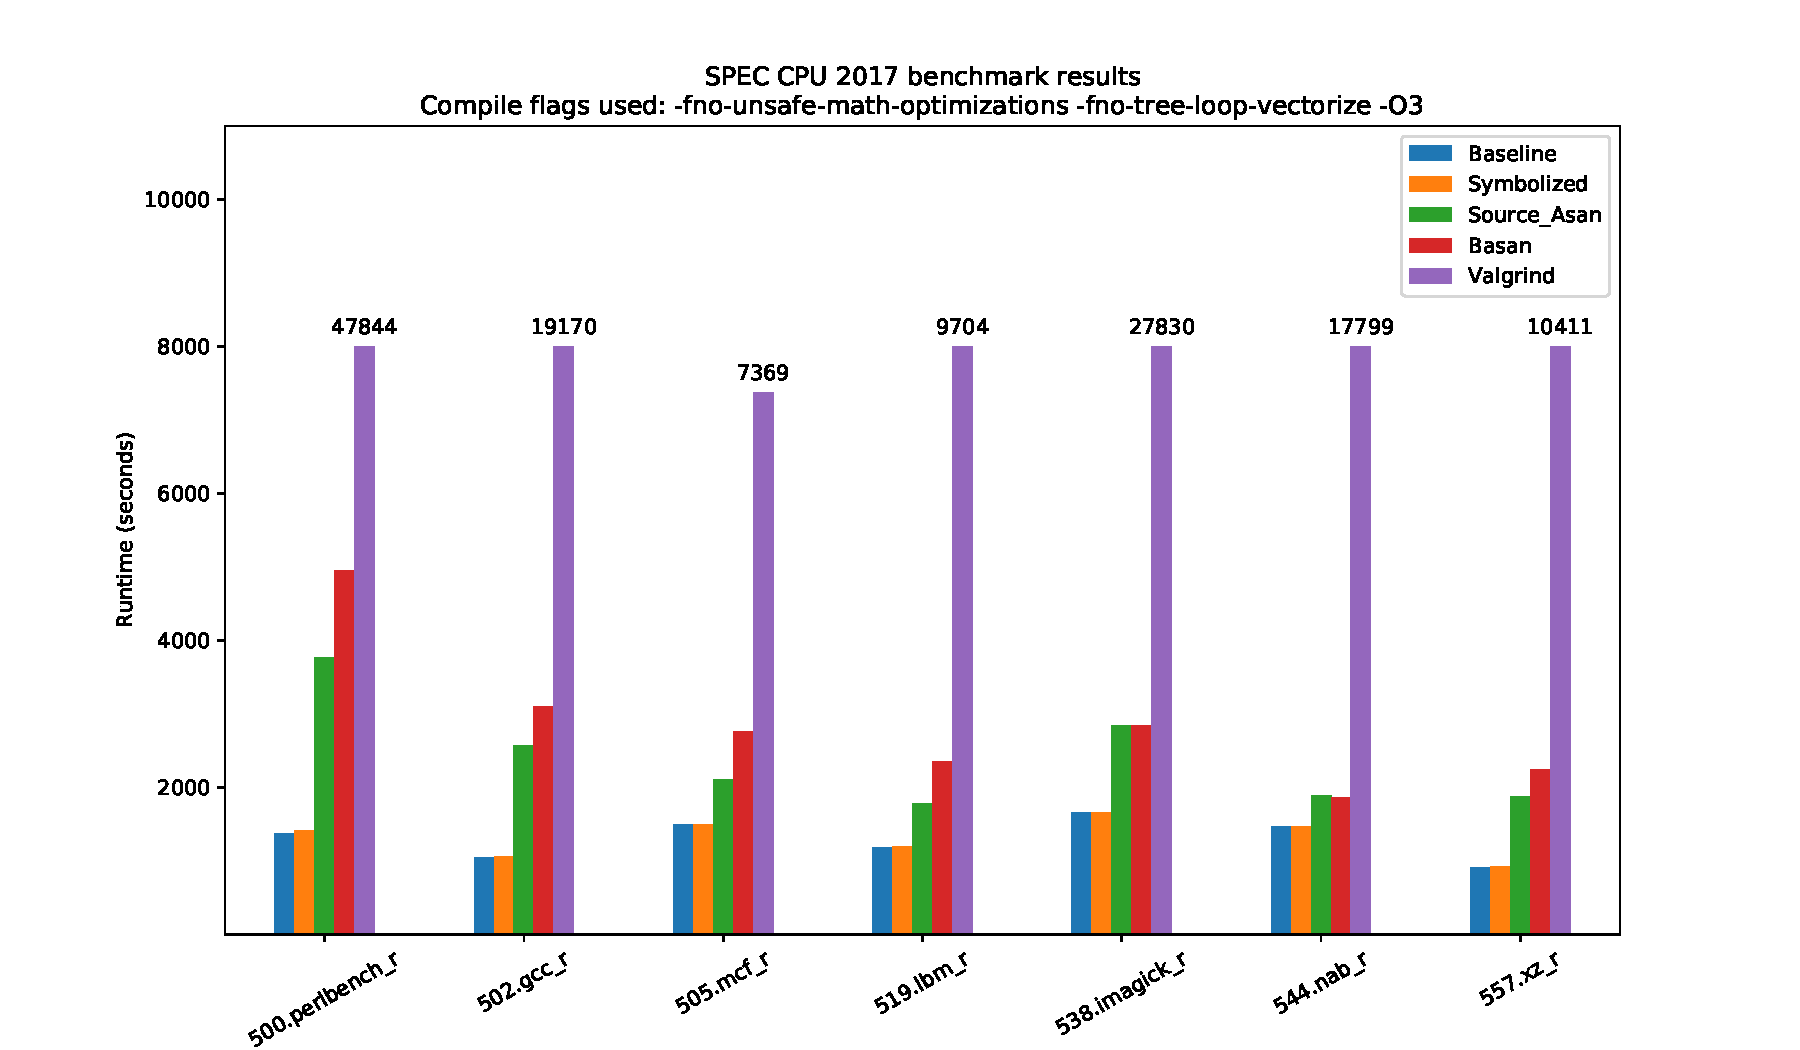
\includegraphics[width=15cm]{cloudlab.pdf}
\centerfloat
	\caption{Benchmark runtime on the Atlas machine. \todo{update plot for new gcc results} } 
\label{plot1}
\end{figure}

\begin{center}
\begin{figure}[h]
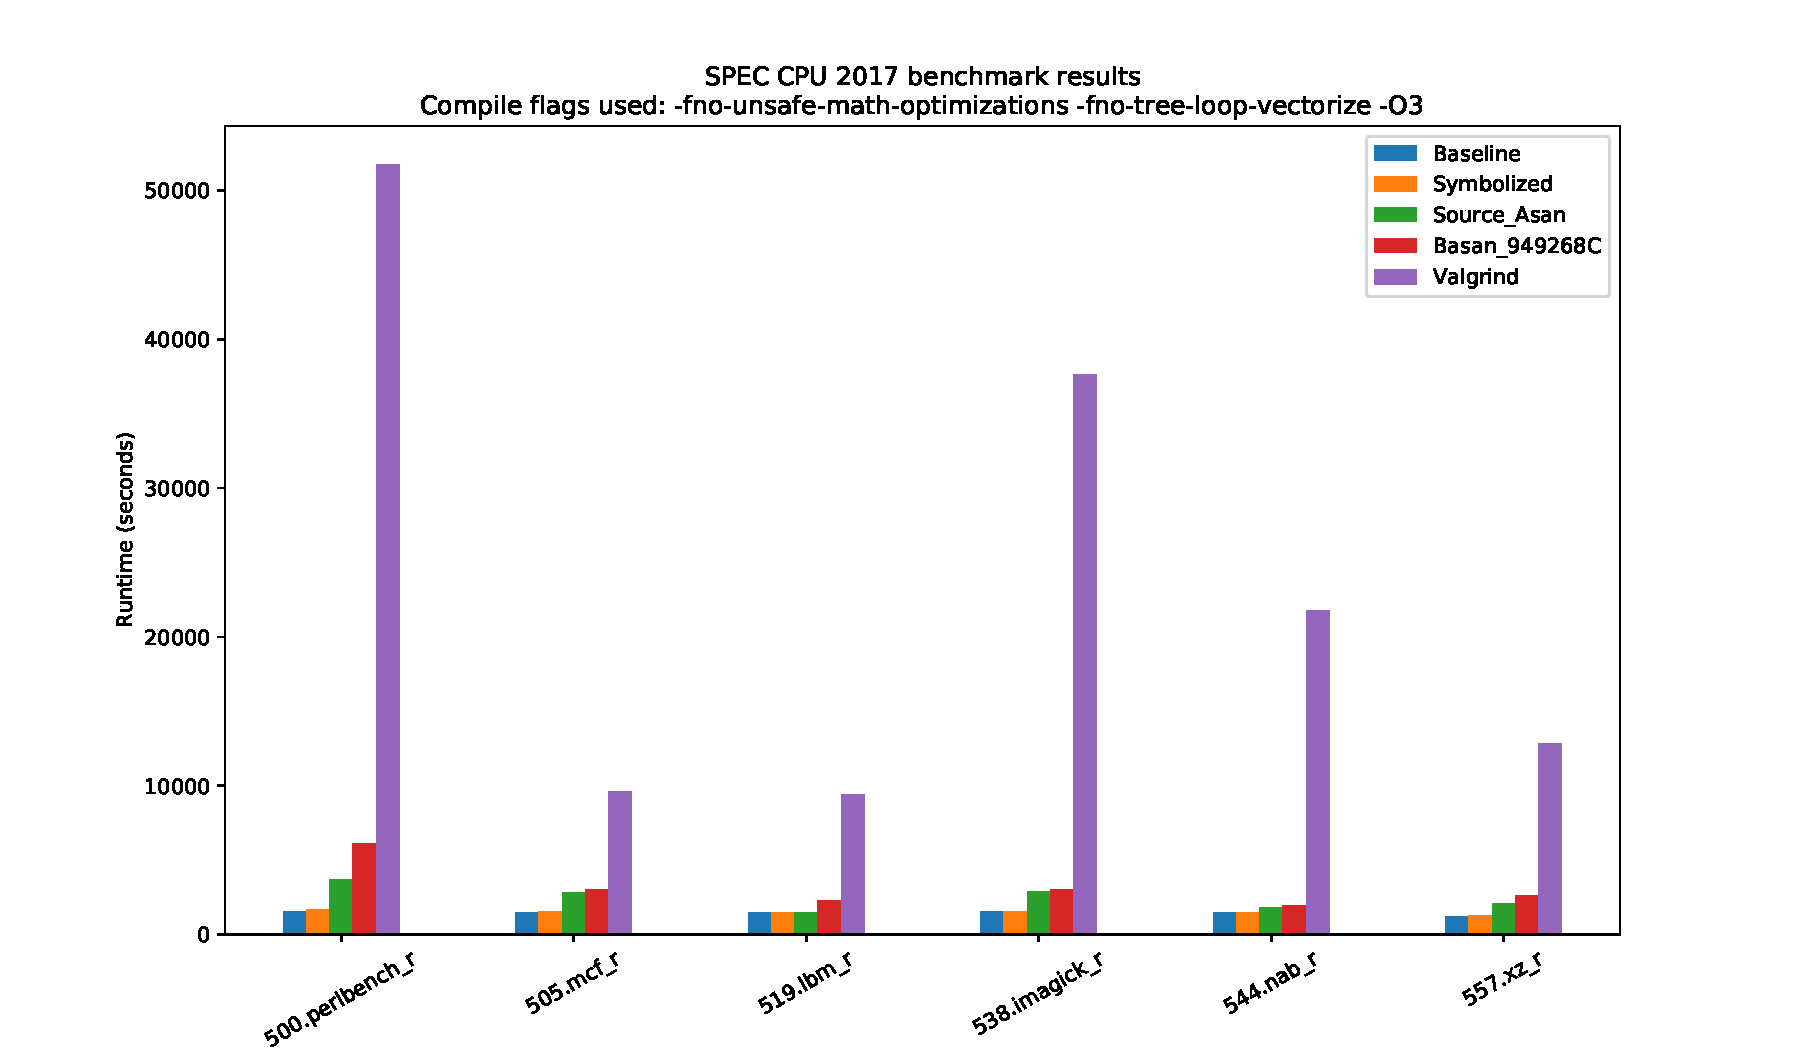
\includegraphics[width=\textwidth]{raspberry.pdf}
\centerfloat
	\caption{Benchmark runtime on the raspberry machine. \todo{LBM SOURCE ASAN time is very strange. seems too low. might want to rerun everything to be extra sure. }}
\label{plot2}
\end{figure}
\end{center}


It's interesting to look at detailed results for the Atlas machine in 
\autoref{labellatabella}. We can see that source-based ASAN has a 84.04\%
overhead on average, but the overhead varies a lot between individual
benchmarks, depending on the amount of memory accesses. For example,
\texttt{perlbench}, running an interpreter, executes a high amount of memory loads
and stores that need to be individually checked by the address sanitizer each
time; in fact, the overhead is noticeably higher (173.84\%). The same holds
true for \sysname's memory sanitization instrumentation (``Binary ASAN'' in
\autoref{labellatabella}): the overhead is larger in programs that frequently
use memory. 

On average, binary ASAN is slower than source ASAN (109.73\% instead of 84.04\%
average overhead \todo{change basan average overhead, incorrect}). The reasons
behind the slowdown are the following:
\begin{itemize}
	\item Number of instrumented locations: Without source code available,
		\sysname cannot use certain types of analysis that the compilers use to 
		determine the safety of certain memory accesses. For this reason, \sysname
		instruments every single memory access, while source ASAN skips some of them.
	\item Assembly generation optimizations: \sysname is a relatively simple tool, 
		and instruments memory accesses with hand-written assembly snippets. While
		some optimizations were implemented (register savings, batching checks), they
		do not even come close to the number and complexity of optimizations passes that
		standard compilers use when generating machine code. 
\end{itemize}
Still, the slowdown with respect to source ASAN is very little compared to
state of the art tools.  In fact, without source code, the only way of adding
memory sanitization to a binary is through dynamic instrumentation. We ran the
benchmarks using a very famous dynamic instrumenter that implements memory
sanitization (Valgrind's \texttt{memcheck} tool~\cite{valgrind}), and plotted
the runtimes in \autoref{plot1} and \autoref{plot2}. The overhead introduced by
dynamic instrumentation is around 10x the overhead of binary ASAN, depending on
the amount of memory accesses of the benchmark. 

\begin{table}
\centerfloat
\begin{tabular}{lrrrr}
\toprule
	\textbf{Name} \hspace{4em} &\textbf{Symbolization only} & \textbf{Source ASAN} & \textbf{Binary ASAN} & \textbf{Valgrind} \\
\toprule

	\texttt{cpugcc\_r   } & 0.95\% &145.80\% &196.09\% & 1729.20\% \\
	\texttt{perlbench\_r} & 2.91\% &173.84\% &260.10\% &3377.03\% \\
	\texttt{imagick\_r}   & 0.30\% & 71.53\% & 71.17\% &1578.53\% \\
	\texttt{nab\_r      } & 0.34\% & 28.57\% & 27.21\% &1110.82\% \\
	\texttt{xz\_r   }     & 0.44\% &105.79\% &144.76\% &1036.57\% \\
	\texttt{mcf\_r      } &-0.07\% & 40.77\% & 83.74\% & 390.94\% \\
	\texttt{lbm\_r      } & 0.59\% & 49.58\% & 97.31\% & 715.46\% \\
	\midrule
	\textbf{Average} & \textbf{0.76\%} & \textbf{84.04\%} & \textbf{119.61\%} & \textbf{1429.94\%} \\
\bottomrule
\end{tabular}
\caption{Overhead of \sysname without instrumentation and of \sysname with
BASAN instrumentation on SPEC CPU2017 on the Atlas machine compared to the original benchmark
and the original benchmarks compiled with source based ASAN.  } 
\label{labellatabella}
\end{table}


However, it needs to be said that our binary ASAN instrumentation has a few
shortcomings. First of all, stack variables access is not instrumented.
Secondly, global variable accesses are not instrumented. Both of those are
caused by the fact that without source code, bounds determination is impossible
for variables in non-heap memory regions. 


\subsection{Optimization: register savings}
One of the biggest performance improvements in our memory sanitization instrumentation 
came from the re-usage of free registers without the need to save them on the stack
at each instrumentation location. 

\autoref{slowregisters} shows the overhead difference in the memory sanitization instrumentation
when register savings are disabled. On average, register savings improved the overhead of
the instrumentation pass by xx.xx\% \todo{THIS EXPERIMENT IS STILL RUNNING}

\begin{table}
\centering
\sisetup{detect-weight=true}
\sisetup{mode=text}
\robustify\bfseries
	\begin{tabular}{lS[table-format=3.2]S[table-format=1.2]}
\toprule
		\textbf{Name} \hspace{4em} & \textbf{Register savings} & \textbf{No registers} \\

\toprule
		\texttt{gcc\_r}       &  196.09\si{\percent} & 259.64  \si{\percent} \\
		\texttt{perlbench\_r} &  260.10\si{\percent} & 453.71  \si{\percent} \\
		\texttt{imagick\_r}   &  71.17 \si{\percent} & 173.40  \si{\percent} \\
		\texttt{nab\_r      } &  27.21 \si{\percent} & 74.22  \si{\percent} \\
		\texttt{xz\_r   }     &  144.76\si{\percent} & 212.01  \si{\percent} \\
		\texttt{mcf\_r      } &  83.74 \si{\percent} & 124.92 \si{\percent} \\
		\texttt{lbm\_r      } &  97.31 \si{\percent} & 99.58  \si{\percent} \\
	\midrule
		\textbf{Average} & \bfseries 119.61\si{\percent} & \bfseries 195.79\% \\
\bottomrule
\end{tabular}
\caption{Overhead of \sysname's memory sanitization with register savings
	turned on or off. On average, the register savings optimization produces code
	with 26.5\% less overhead.}
\label{slowregisters}
\end{table}


\subsection{Comparison to trampolines}

Trampolines are one of the most straight-forward way to instrument a binary, and they are
are free from the burden of static analysis required to perform symbolization. However, we
would like to show that the tradeoff in performance is very large compared to the in-place
instrumenation that symbolization permits to do. 

We implemented the same memory sanitization instrumentation pass by using
trampolines, and ran the benchmarks with it to compare the timings. Results can
be seen in \autoref{slowtrampolines}. 

This was a fairly simple experiment that used only a single type of very heavy instrumenation
(memory sanitization adds a lot of branches in the code and a very large number of 
instructions need to be instrumented), but the difference in overhead is very large, with
trampolines being 56\% slower on average compared to symbolized in-place instrumentation. 
We expect lower differences in overhead when using lighter forms of instrumentation, but not
enough lower to avoid being noticeable. 



\begin{table}
\centering
\sisetup{detect-weight=true}
\sisetup{mode=text}
\robustify\bfseries
	\begin{tabular}{lSS[table-format=1.2]S[table-format=3.2]}
\toprule
		\textbf{Name} \hspace{4em} & \textbf{Binary ASAN} & \textbf{Trampoline ASAN} \\

\toprule
		\texttt{perlbench\_r} &  260.10 \si{\percent} & 636.41  \si{\percent} \\
		\texttt{imagick\_r}   &  71.17  \si{\percent} & 188.96  \si{\percent} \\
		\texttt{nab\_r      } &  27.21  \si{\percent} & 77.82  \si{\percent} \\
		\texttt{xz\_r   }     &  144.76 \si{\percent} & 232.64  \si{\percent} \\
		\texttt{mcf\_r      } &  83.74  \si{\percent} & 135.31 \si{\percent} \\
		\texttt{lbm\_r      } &  97.31  \si{\percent} & 104.79  \si{\percent} \\
	\midrule
		\textbf{Average} & \bfseries 109.73\% & \bfseries 227.38\% \\
\bottomrule
\end{tabular}
\caption{Overhead of \sysname's in-place instrumentation and trampoline-based
	instrumentation using memory sanitization as the instrumentation pass. On average, 
	trampolines are 56\% slower than in-place instrumentation.}
\label{slowtrampolines}
\end{table}




\section{Correctness}

While the SPEC CPU benchmark checks the validity of the output of each benchmark
that is run, we decided that we wanted further proof of the correctness of our
approach with more widely used and common binaries. For this reason, we selected
the coreutils suite of tools, and ran their tests on the binaries rewritten
with \sysname. 

We used the release 8.32 package downloaded from
\url{https://ftp.gnu.org/gnu/coreutils/}. We first built the binaries using
\texttt{make}, then rewrote every single one of them two times: first, without
instrumentation, and then with memory sanitization enabled. We then ran
the extensive version of their testsuite with \texttt{make check-very-expensive}. 

The results of the tests can be seen in \autoref{coreutils}. Of the 4 failed
tests with memory sanitization turned on, two of them are caused by the
testsuite trying to \texttt{LD\_PRELOAD} libraries (which is not compatible
with AddressSanitizer) in the \texttt{stdbuf} tests, and the other two are
because of the overhead of the instrumentation that triggers a timeout in the
tests.




\begin{table}
\centering
\begin{tabular}{lrr}
\toprule
	& \textbf{Symbolization only} & \textbf{Binary ASAN} \\
\toprule
	Total              & 621 & 621 \\
	Passed              & 540  & 536  \\
	Skipped              & 81  & 81  \\
	Failed              & 0  & 4  \\
\bottomrule
\end{tabular}
\caption{Results of the coreutils ``very expensive'' test suite on binaries rewritten through \sysname, comparing memory sanitization enabled or disabled. The skipped tests are due to uninstalled third-party dependencies, or architecture specific features missing on the Raspberry.}
\label{coreutils}
\end{table}



\section{Comparison with Egalito}
The only state-of-the-art rewriter engine that had features comparable to
\sysname is Egalito~\cite{egalito}. Egalito is a binary ``recompiler'' targeted
at C, position-independent Linux executables that lifts binary to a custom
Intermediate Representation (IR) and supports a large variety of
instrumentation and transformation passes, and has a (reported) similar
baseline overhead to \sysname (0.46\% on SPEC CPU2006). The comparison with
Egalito is interesting because the authors had to tackle very similar problems
as ours (pointer construction and jump table recovery); however, they do not
address how they solved the problem of jump table enlargement in the case of
heavyweight instrumentation.  Unfortunately, we were not able to perform any
kind of comparison as the latest version available in the public repository
crashes on any \texttt{aarch64} binary we tried to recompile. We opened an
issue \footnote{\url{https://github.com/columbia/egalito/issues/32}} on their
public Github repository on November 28, 2020, but it still left unanswered (as of \today).



\todo{Do we want to talk about cache misses? I already have scripts to measure them, I just need to 
run all the benchmarks all over again}
\mat{If you have them sure, but as lower priority. Nice to have but not a must.}



%%%%%%%%%%%%%%%%%%%%%%
\chapter{Related Work}
%%%%%%%%%%%%%%%%%%%%%%

%The related work section covers closely related work. Here you can highlight
%the related work, how it solved the problem, and why it solved a different
%problem. Do not play down the importance of related work, all of these
%systems have been published and evaluated! Say what is different and how
%you overcome some of the weaknesses of related work by discussing the 
%trade-offs. Stay positive!
%This section is usually 3-5 pages.


% useful links:
% REPICA: https://ieeexplore.ieee.org/stamp/stamp.jsp?arnumber=8454360
%         good state of the art overview, both ARM64 and arm32
%         1. do not use symbolization, but relative address correction
%         2. Detect jump tables and global pointers, but not fix them
%         3. Overhead is exactly the same as retrowrite
% A SURVEY ON BINARY REWRITING: https://publications.sba-research.org/publications/201906%20-%20GMerzdovnik%20-%20From%20hack%20to%20elaborate%20technique.pdf

{

\setlength{\parindent}{0cm}

\todo{This section now has only list of related work I would like to talk 
about, will be expanded later}


\todo{Complain about egalito}



\textbf{Dynamic rewriters in general}:\\
First, the good ol' ones: \texttt{PIN}~\cite{pin}, 
\texttt{Valgrind}~\cite{valgrind} and \texttt{DynInst}~\cite{dyninst}.

More recently, \texttt{Multiverse}~\cite{multiverse}, \texttt{Frida} and 
\texttt{DynamorIO} are interesting examples.

\texttt{QASAN}~\cite{qasan} is similar to \sysname's BASan, much slower but 
also much more portable (works on any binary supported by QEMU)



\textbf{Static rewriters that use lifting to IR}:\\
\texttt{McSema}~\cite{mcsema} is a great example of LLVM IR lifting approach, 
also particularly nice as it supports C++ exceptions

\textbf{Static rewriters that use trampolines}:\\
\texttt{E9patch}~\cite{e9patch} uses only trampolines, no need to recover 
control flow, but also noticeable overhead

%\todo{Also say that trampolines are especially effective on ARM because every 
%instruction is always 4 bytes, so you don't need to worry about overwriting 
%instructions shorter than a jmp like in x86}

\textbf{Static rewriters that use symbolization}:\\
\texttt{Uroboros}~\cite{uroboros} and \texttt{Ramblr}~\cite{ramblr} are the 
first reassemblable assembly approaches (symbolization), 
\sysname~\cite{dinesh20oakland} (x86 version)

\textbf{Static rewriters aimed at ARM binaries}:\\
\texttt{Repica}~\cite{repica} is probably the most recent addition to binary 
rewriters aimed at ARM binaries.  

\todo{Discuss Bistr?}~\cite{bistro}

For more check out recent surveys on the area of binary rewriting~\cite{binaryrewritingsurvey}

}

%%%%%%%%%%%%%%%%%%%%%
\chapter{Future Work}
%%%%%%%%%%%%%%%%%%%%%

{

\setlength{\parindent}{0cm}
\hangindent=0.7cm \textbf{Support for more source languages}: For now, 
\sysname supports only binaries compiled from the C language, both for the 
\texttt{x86} and the ARM implementation. The easiest addition would be to add 
support for C++ by expanding the analysis capabilities of \sysname to support 
exception tables too, but many more languages could be supported in the future. 

\hangindent=0.7cm \textbf{Support for kernel space binaries}: Right now the ARM 
port of \sysname supports only userspace binaries, contrary to the 
\texttt{x86} version that supports linux kernel modules too. The kernel version 
of \sysname\_ARM would prove to be particularly interesting as it would open 
new ways to efficiently fuzz Android kernel modules.

\hangindent=0.7cm \textbf{Support for more executable formats/operating 
systems}: The current implementation of the \sysname tool is aimed only 
towards ELF files, but adding support for MACH-O and PE binaries should not 
require too much effort. This would also be interesting as Windows and MacOS 
present way more closed-source modules compared to Linux.

\hangindent=0.7cm \textbf{More instrumentation passes}: While right now we 
implemented only the AddressSanitizer instrumentation in the ARM port of
\sysname, the design of \sysname is modular and adding new instrumentation 
passes or new mitigations should be easy. To name a few, the interesting ones would be:
\begin{itemize}
	\item Shadow stack (return address protection)
	\item Control flow authentication using ARM pointer authentication 
		(hardware-assisted)
	\item Coverage-guidance for fuzzing
\end{itemize}

}

%%%%%%%%%%%%%%%%%%%%
\chapter{Conclusion}
%%%%%%%%%%%%%%%%%%%%


In summary, we develop the ARM architecture implementation of the \sysname 
project, a scalable static rewriter for linux C binaries.  \sysname enables 
targeted application of static instrumentation where no source code is 
available, such as proprietary binaries, inline assembly, or code generated by 
a deprecated compiler.  We also present an example instrumentation pass on top 
of the symbolization engine, AddressSanitizer, particularly useful for fuzzing 
purposes. We present new solutions to problems arising from the peculiarities 
of the ARM architecture such as the fixed-size instruction set, global variable 
accesses and jump table instrumentation. We show that the total overhead of the 
symbolization and the instrumentation pass are competitive with source based 
AddressSanitizer.  Our work shows that \sysname's original approach is not 
limited to the \texttt{x86} architecture, but can be applied to the ARM 
architecture and more.



\cleardoublepage
\phantomsection

\addcontentsline{toc}{chapter}{Bibliography}
\printbibliography

% Appendices are optional
% \appendix
% %%%%%%%%%%%%%%%%%%%%%%%%%%%%%%%%%%%%%%
% \chapter{How to make a transmogrifier}
% %%%%%%%%%%%%%%%%%%%%%%%%%%%%%%%%%%%%%%
%
% In case you ever need an (optional) appendix.
%

\end{document}



\appendix

\input{appendix}

\backmatter

\bibliographystyle{plain}
%\bibliography{thesis}

\includepdf[pages={-}]{declaration-originality.pdf}

\end{document}
